\documentclass[%
 reprint,
superscriptaddress,
%groupedaddress,
%unsortedaddress,
%runinaddress,
%frontmatterverbose, 
%preprint,
%preprintnumbers,
nofootinbib,
%nobibnotes,
%bibnotes,
 amsmath,amssymb,
 aps,
 pra,
%prb,
%rmp,
%prstab,
%prstper,
%floatfix,
]{revtex4-2}
\usepackage{graphicx} % Required for inserting images
\usepackage{pgfplotstable}
\usepackage{booktabs}
\usepackage{siunitx}
\usepackage{float}
\restylefloat{table}

\usepackage[hyperfootnotes=false,colorlinks=true]{hyperref}
\hypersetup{
    linkcolor=black,           % Use text color for internal links
    citecolor=blue,        % Keep citations colored (optional)
    urlcolor=blue,         % Keep URLs colored (optional)
    pdfborder={0 0 1}      % Remove all borders/boxes
}

\makeatletter 
\renewcommand\onecolumngrid{%
\do@columngrid{one}{\@ne}%
\def\set@footnotewidth{\textwidth}% <<<< Use full text width
\def\footnoterule{\kern-6pt\hrule width \textwidth\kern6pt}% <<<< Full width rule
}
\renewcommand\twocolumngrid{%
        \def\set@footnotewidth{\textwidth}% <<<< Key change: use full text width
        \def\footnoterule{% Full width rule for two-column mode
        \dimen@\skip\footins\divide\dimen@\thr@@
        \kern-\dimen@\hrule width \textwidth\kern\dimen@}% <<<< Changed from .5in to \textwidth
        \do@columngrid{mlt}{\tw@}
}%
% Additional patch to ensure footnotes actually use the full width
\long\def\@footnotetext#1{%
  \insert\footins{%
    \reset@font\footnotesize
    \interlinepenalty\interfootnotelinepenalty
    \splittopskip\footnotesep
    \splitmaxdepth \dp\strutbox \floatingpenalty \@MM
    \hsize\textwidth% <<<< Force footnotes to use full text width
    \@parboxrestore
    \protected@edef\@currentlabel{%
       \csname p@footnote\endcsname\@thefnmark
    }%
    \color@begingroup
      \@makefntext{%
        \rule\z@\footnotesep\ignorespaces#1\@finalstrut\strutbox}%
    \color@endgroup}}%
\makeatother

\begin{document}

\title{BBN Uncertainties with Gaussian Processes}
\author{Tim Launders}
\affiliation{Boston University}

\date{\today}

\maketitle
\setlength{\parskip}{8pt}

\onecolumngrid

\section{Introduction}



With experimental constraints of primordial element abundances reaching percent-level precision\footnote{Need sources for this for both D/H and Y$_\text{P}.$}, theoretical predictions must be rigorously analyzed to achieve similar precision. Using a novel approach with Gaussian processes, this work directly incorporates experimentally reported nuclear reaction data and uncertainties (both statistical and systematic) into primordial element abundance calculations. 

The complicated nature of the strong force makes theoretical calculations for these reactions very difficult, even with a few interacting nucleons; therefore, experimental data should be incorporated into BBN calculations as directly as possible. Two leading BBN codes, PRIMAT \cite{Pitrou2018} and PArthENoPE \cite{Gariazzo2022}, use different techniques to fit experimental nuclear reaction data. For reactions in PRIMAT, theoretical calculations are scaled to fit data in a fully Bayesian framework. On the other hand, the reactions in PArthENoPE are fit with a low-degree polynomial. For some reactions, they yield different central values for rates, which propagate to a discrepancy in the predicted deuterium abundance of $\sim2\sigma$. Both estimate the uncertainties in primordial abundances\footnote{Should look into exactly how these uncertainties are handled when factoring in other error sources.} due to uncertainties in the reaction rates by shifting them by $1\sigma$.

The three deuterium burning reactions -- $d$($d$,$n$)$^3$He, $d$($d$,$p$)$t$, and $d$($p$,$\gamma$)$^3$He -- have the greatest influence on primordial deuterium. Since the methods employed for PRIMAT and PArthENoPE disagree on the deuterium abundance while lying within experimental constraints for the helium-4 abundance, these reactions are selected for this analysis. 

Using Gaussian processes for these fits provides several benefits. (1) Passing function samples from the Gaussian process posterior through the BBN code (in this case, LINX) provides robust uncertainties on primordial abundances. (2) Assumptions regarding the functional form of reaction rates are relaxed from exact expressions to general properties that these functions are expected to follow, expanding the space of functions allowed by the data. (3) By not fixing an exact functional form, more freedom is allowed in energy regions with few or no data points, giving strong uncertainty estimates in these regions. (4) Systematic uncertainties are directly incorporated within the Gaussian process framework. (5) Gaussian process regression can be performed either with a purely data-driven approach or by using \textit{ab initio} theoretical calculations as a prior. 

This note outlines the current status of this work. Section 2 outlines the Gaussian process regression process for the deuterium burning reactions. The resulting abundance predictions are presented and analyzed in section 3. Section 4 discusses outstanding questions that are left for future work. The remaining sections provide further details omitted earlier. 




\section{Methods}



Nuclear cross sections as a function of center of mass energy $\sigma(E)$ are measured in labs, typically using a fixed-target collider. Due to the Coulomb repulsion between nuclei, cross sections typically span many orders of magnitude; it is convenient to express the cross section in terms of the astrophysical S-factor
\begin{equation}
	S(E) = \sigma(E) E e^{2\pi\eta},
\end{equation}
where $\eta = \hbar^{-1}\sqrt{\frac{\mu}{2E}}Z_0 Z_1 e^2$ is the Sommerfeld parameter \cite{Iliadis2015}. $\mu$ is the reduced mass of the two-body system, and $Z_0$ and $Z_1$ are the charges of the two nuclei. The exponential term (the Gamow factor) is the leading order term for the $\ell=0$ transmission coefficient in a Coulomb potential. Thermally-averaging the S-factor using a Maxwell-Boltzmann distribution gives the reaction rate:
\begin{equation}
	R(T) \equiv N_A \langle \sigma v \rangle = \sqrt{\frac{8}{\pi \mu}} \frac{N_A}{(k_B T)^{3/2}} \int_{0}^{\infty} dE \, e^{-2 \pi \eta} S(E) e^{-E/k_B T}.
\end{equation}

To use Gaussian processes here, certain assumptions must be made. All reported uncertainties in input datasets are assumed to follow Gaussian statistics\footnote{Perhaps we want to elaborate on this point and show why this is a reasonable assumption.} and to be accurate representations of the uncertainty in each measurement. In line with the literature, \textbf{systematic errors within each dataset are assumed to affect each data point in the same way}, shifting each point up or down by the same (percent) amount. To incorporate these assumptions within the Gaussian process framework, the covariance matrix of the input datasets is added to the upper-left block of the partitioned full covariance matrix, in the same spirit as the widely used procedure of adding statistical errors to the diagonal. 

Any kernel choice includes assumptions about the latent function. The kernel encodes correlations between S-factor values at different energies; a simple, common kernel choice is the squared exponential\footnote{The squared exponential kernel is often referred to as the RBF (radial basis function) kernel.} \cite{Rasmussen2006}
\begin{equation}
	k_{SE}(d) = e^{\frac{-d^2}{2\ell^2}} \nonumber
\end{equation}
where $\ell$ is a hyperparameter representing the characteristic length scale of correlations in input space and $d$ is the distance between two points in input space. When the latent function is expected to be smooth throughout input space with correlations that only depend on the distance between points in input space, the squared exponential is an appropriate kernel choice. The Mat\'ern class of kernels relaxes the smoothness assumption while still including a characteristic length scale in a similar manner:
\begin{equation}
	k_{M,\nu}(d) =  \frac{2^{1-\nu}}{\Gamma(\nu)} \left( \frac{\sqrt{2\nu} d}{\ell} \right)^\nu K_\nu\left( \frac{\sqrt{2\nu} d}{\ell} \right), \nonumber
\end{equation}
where $K_\nu$ is the modified Bessel function of the second kind \cite{Rasmussen2006}. $\nu$ is a positive parameter that controls the smoothness of functions drawn from the Gaussian process posterior. A smaller $\nu$ gives less smooth functions, and the Mat\'ern kernel becomes the squared exponential in the limit $\nu\to\infty$. 

Kernel choices for this application should yield S-factor functions that do not strongly deviate from leading theoretical calculations with uncertainties that are reasonable given reported experimental uncertainties. Sampled S-factor functions are expected to be globally smooth, as deuterium burning reactions have no resonances in the relevant energy range. This observation suggests that the squared exponential kernel would work well; however, a Mat\'ern kernel must be added to the squared exponential to fit these criteria. With only the squared exponential kernel, the fit is driven to a small correlation amplitude and length scale since the Gaussian process assumes that all points are drawn from the same latent function. When multiple perfectly correlated datasets have data points at very similar energies that differ by $>1\sigma$, there are two options for the Gaussian process: either some of the datasets are multiple $\sigma$ off from the latent function, or the latent function itself contains small-scale fluctuations. During hyperparameter optimization, a small characteristic length scale for the squared exponential kernel is chosen, being more probable than datasets being off by multiple $\sigma$. The addition of a small-$\nu$ ($\nu<1$) Mat\'ern kernel allows the model to fit these small-scale fluctuations while accommodating the global shape provided by the squared exponential kernel. Therefore, the following kernel form\footnote{This notation feels super clunky...} is used for the deuterium burning reactions: 
\begin{equation}
	k(d) = \alpha \, k_{SE}(d, \ell_1) + \beta \, k_{M, 1/4}(d, \ell_2) \nonumber
\end{equation}
with four hyperparameters -- two constants controlling the amplitude of correlations ($\alpha$ and $\beta$) and two characteristic length scales ($\ell_1$ and $\ell_2$). This kernel choice implicitly assumes that correlations only depend on differences in energies. Whenever any kernel is used in this work, \textbf{log energies are used}. 

Hyperparameters are selected using ``Leave-Dataset-Out'' (LDO) optimization, a form of cross-validation in which each dataset is withheld from the rest. The model is evaluated on its performance on the unseen dataset\footnote{Details for this method are in section 5.}. The \textit{Adam} optimizer \cite{Kingma2017} is used for gradient descent to avoid convergence to a local minimum. Optimization is considered converged when the step size drops below $10^{-5}$. A common optimization technique, in which the marginal likelihood to observe all of the data points is maximized, is also considered for comparison. Two different prior mean functions are considered for the S-factor: an uninformative prior that is zero everywhere and the theoretical calculations used in PRIMAT. 

Once the model has been fit to the experimental data, sample functions are drawn from the posterior and integrated at a discretized interval of temperatures using (2) to get the rate distribution. These rate samples are directly used in LINX \cite{Giovanetti2024}. The mean and standard deviation of the rate distribution at each temperature give the $1\sigma$ envelopes shown in subsequent plots.

\subsection{d(d,n)$^3$He}

Figure 1 shows four plots to analyze the Gaussian process fit to $d$($d$,$n$)$^3$He S-factor data. The model fit using the a zero mean prior and LDO hyperparameter optimization is shown in all plots. The posterior mean is somewhat jagged in some regions from the contribution of the Mat\'ern kernel component, while the smoothness from the squared exponential kernel component dominates at higher energies. If the data preferred this smooth behavior at all energies, the constant hyperparameter multiplying the Mat\'ern component would have been driven to zero. Individual sample draws have more jagged small-scale fluctuations than the mean, but rate draws are smooth when integrated. These small-scale fluctuations are a product of requiring the small-$\nu$ Mat\'ern component in the kernel to capture correlations. S-factor uncertainties are comparable to reported experimental uncertainties and increase slightly in regions with without any data points. The overall shape is comparable with the theoretical prediction, notably between 0.3-0.8 MeV where there are no data. The Gaussian process $1\sigma$ rate envelope is around 1.5\% in the relevant temperature range for BBN, slightly larger than those of both PRIMAT and PArthENoPE. 

The Gaussian process mean lies closest to the BR90 dataset \cite{Brown1990} (shown in blue) in the energy range with overlapping datasets, as expected since this dataset has the smallest reported uncertainties. Additionally, each of the higher energy points in the KR87M dataset \cite{Krauss1987} (shown in green) lie below the Gaussian process mean by the same percentage. This suggests that this technique handles correlations as desired since these points have negligible statistical uncertainty. The fit is mostly insensitive to the choice of mean prior and hyperparameter optimization; using the theoretical prediction for the prior mean and optimizing the marginal likelihood make very little impact on the fit. The most impactful difference when using the marginal likelihood comes between 0.03 and 0.1 MeV, where the Gaussian process mean is consistently very slightly lower than the other two correlated Gaussian process means, resulting in a slightly lower rate\footnote{Seen in the next section this translates to a slightly higher predicted value of D/H.}. However, excluding correlations from the model entirely makes a meaningful impact, aligning the fit more closely with that from PArthENoPE. Perhaps this suggests that fitting a higher degree polynomial with their method would indeed have little impact on the fit, and some aspect of their handling of systematic uncertainties is insufficient\footnote{This is a big claim...it is also possible that the assumption of systematics shifting each data point up or down by the same amount is flawed, making PArthENoPE's method more accurate. Their predicted deuterium abundance is closer to the observed value. \phantom{Some text to help with formatting}}. 

Both the S-factor and rate agree more closely with those used in PRIMAT, despite Gaussian process regression seeming more similar to fitting a polynomial. However, the Gaussian process has much greater flexibility in fitting the data than a polynomial, and the data prefer a fit that is more similar to the theoretical calculation regardless of the prior mean choice. 

\begin{figure}
    	\centering
    	\begin{minipage}{.48\textwidth}
        		\centering
        		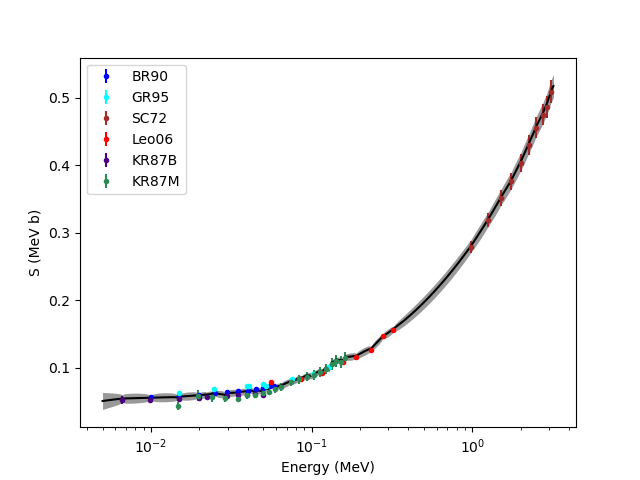
\includegraphics[width=\linewidth]{Figures/ddhe3n_S.png}
    	\end{minipage}
    	\hspace{0mm}
    	\begin{minipage}{.48\textwidth}
        		\centering
        		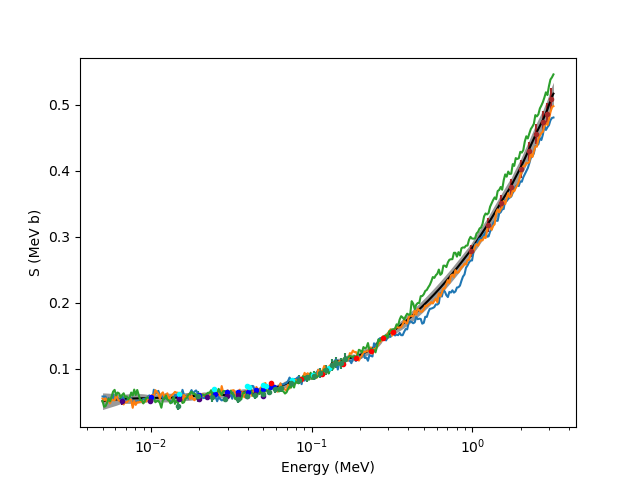
\includegraphics[width=\linewidth]{Figures/ddhe3n_S_samples.png}
    	\end{minipage}
    	\begin{minipage}{.48\textwidth}
    		\centering
		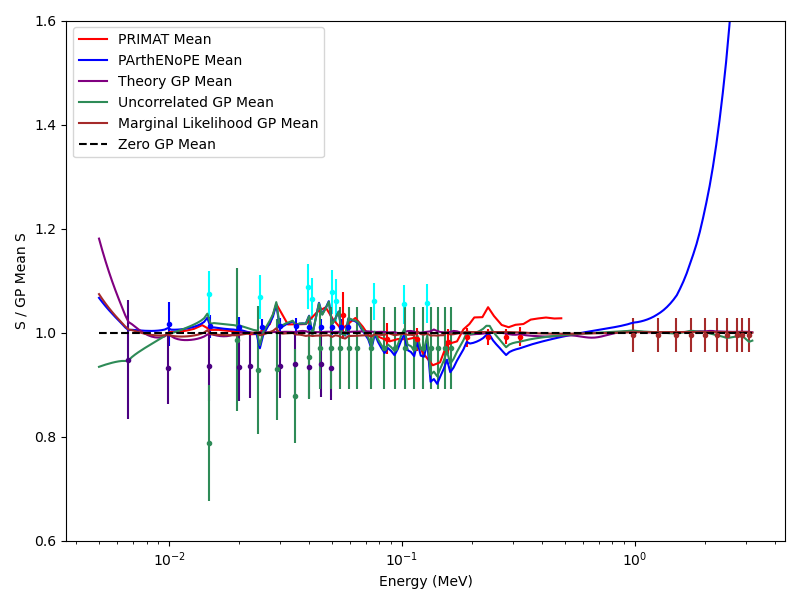
\includegraphics[width=\linewidth]{Figures/ddhe3n_S_comp.png}	
	\end{minipage}
	\hspace{0mm}
	\begin{minipage}{.48\textwidth}
    		\centering
		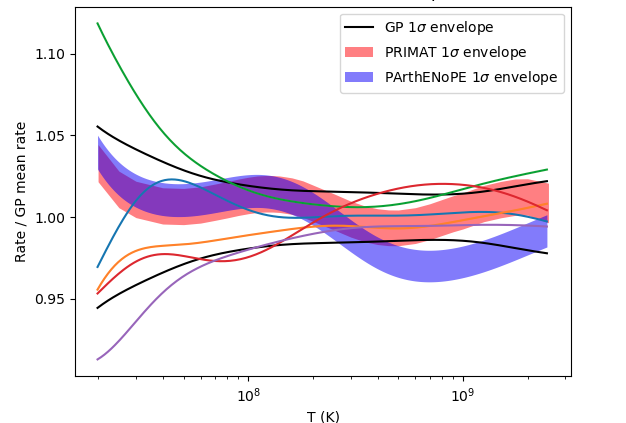
\includegraphics[width=\linewidth]{Figures/ddhe3n_rate.png}	
	\end{minipage}
    	\caption{Gaussian process regression fits to $d$($d$,$n$)$^3$He S-factor data. \textit{Top left}: Gaussian process mean and $1\sigma$ envelope in the BBN energy range. An uninformative zero prior mean and LDO hyperparameter optimization are used. The six datasets \cite{Schulte1972, Krauss1987, Brown1990, Greife1995, Leonard2006} used to fit the model are shown with $1\sigma$ total error bars. \textit{Top right}: Three samples drawn from the posterior overlayed on the mean and $1\sigma$ envelope. \textit{Bottom left}: Three additional Gaussian process means -- one using the \textit{ab initio} theoretical calculation from \cite{Arai2011} as the prior mean, one excluding correlations within datasets, and one using marginal likelihood hyperparameter optimization -- as well as the fits used by PRIMAT and PArthENoPE, normalized to the fit above. \textit{Bottom right}: Gaussian process S-factor fit in the top plots integrated to get the reaction rate, along with the rates from PRIMAT and PArthENoPE. 5 samples drawn from the posterior are shown. }
\end{figure}

\subsection{d(d,p)t}

Figure 2 shows four plots to analyze the Gaussian process fit to $d$($d$,$p$)$t$ S-factor data. As with $d$($d$,$n$)$^3$He, the model fit using the a zero mean prior and LDO hyperparameter optimization is shown in all plots. Many qualities of this reaction are similar to those of $d$($d$,$n$)$^3$He as five of the six experiments used in each are the same. Without the highest energy dataset of $d$($d$,$n$)$^3$He, the uncertainties grow much more significantly after $\sim0.3$ MeV. However, the addition of GR95C (shown in brown) greatly constrains the fit at low energies. The PRIMAT fit does not include this dataset, driving the Gaussian process fit above that of PRIMAT in this region. Again, the addition of the Mat\'ern component to the kernel makes the mean and subsequent sample draws jagged with small-scale fluctuations that become smooth after integration. S-factor uncertainties are reasonable given the reported experimental uncertainties, and the shape of the Gaussian process mean is comparable with the theoretical prediction. It is somewhat interesting that after 0.3 MeV, where there are no longer experimental data, the Gaussian process mean does not collapse to the zero prior mean and continues to increase. The Gaussian process $1\sigma$ rate envelope is around 1.1\% in the relevant temperature range for BBN, comparable in size to those of PRIMAT and PArthENoPE.

The Gaussian process mean again lies closest to those datasets with smallest error bars, and correlations can be seen in the same way as with $d$($d$,$n$)$^3$He in the normalized S-factor plot. The fit is more sensitive to use of the theory mean prior, but only at the lowest and highest energies where there are no data. The uncorrelated Gaussian process mean is not as similar to the fit from PArthENoPE, but is still similar between 0.01-0.09 MeV. Between 0.02 and 0.3 MeV the Gaussian process means match the PRIMAT fit very well, which is reflected in the rate envelopes. Again, the data prefer a fit that is more similar to the theoretical calculation regardless of prior mean choice.

\begin{figure}
    	\centering
    	\begin{minipage}{.48\textwidth}
        		\centering
        		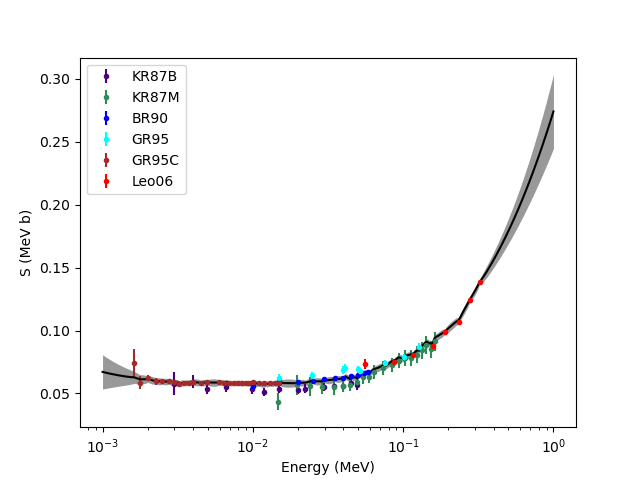
\includegraphics[width=\linewidth]{Figures/ddtp_S.png}
    	\end{minipage}
    	\hspace{0mm}
    	\begin{minipage}{.48\textwidth}
        		\centering
        		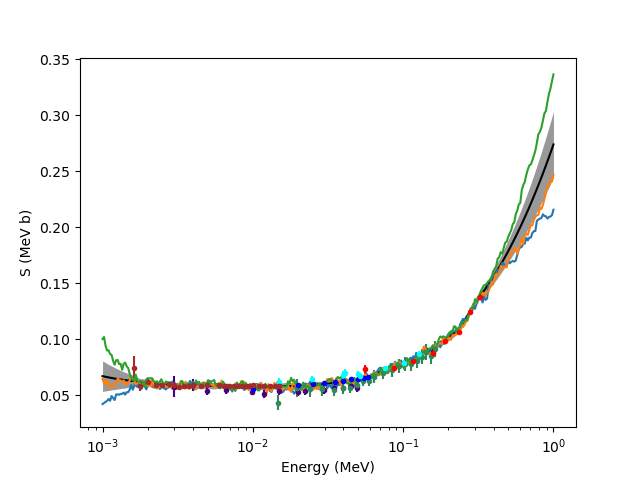
\includegraphics[width=\linewidth]{Figures/ddtp_S_samples.png}
    	\end{minipage}
    	\begin{minipage}{.48\textwidth}
    		\centering
		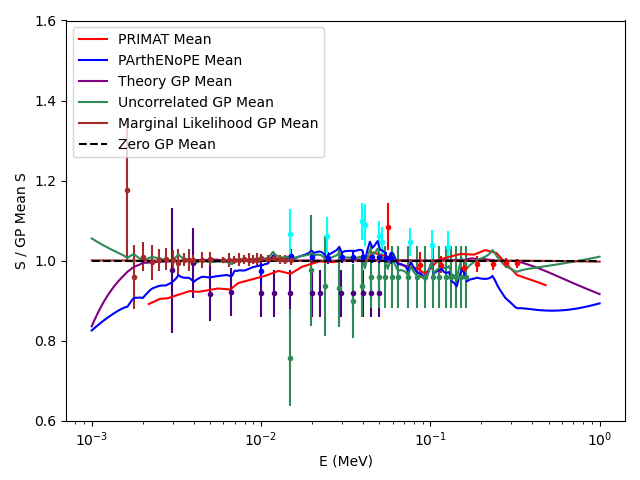
\includegraphics[width=\linewidth]{Figures/ddtp_S_comp.png}	
	\end{minipage}
	\hspace{0mm}
	\begin{minipage}{.48\textwidth}
    		\centering
		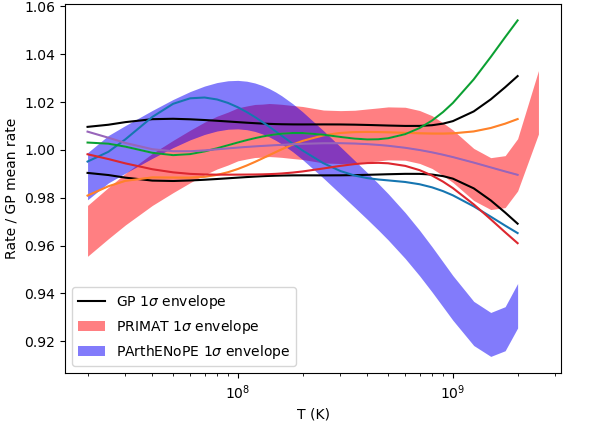
\includegraphics[width=\linewidth]{Figures/ddtp_rate.png}	
	\end{minipage}
    	\caption{Gaussian process regression fits to $d$($d$,$p$)$t$ S-factor data. \textit{Top left}: Gaussian process mean and $1\sigma$ envelope in the BBN energy range. An uninformative zero prior mean and LDO hyperparameter optimization are used. The six datasets \cite{Krauss1987, Brown1990, Greife1995, Leonard2006} used to fit the model are shown with $1\sigma$ total error bars. \textit{Top right}: Three samples drawn from the posterior overlayed on the mean and $1\sigma$ envelope. \textit{Bottom left}: Three additional Gaussian process means -- one using the \textit{ab initio} theoretical calculation from \cite{Arai2011} as the prior mean, one excluding correlations within datasets, and one using marginal likelihood hyperparameter optimization -- as well as the fits used by PRIMAT and PArthENoPE, normalized to the fit above. \textit{Bottom right}: Gaussian process S-factor fit in the top plots integrated to get the reaction rate, along with the rates from PRIMAT and PArthENoPE. 5 samples drawn from the posterior are shown. }
\end{figure}

\subsection{d(p,$\gamma$)$^3$He}

Fitting a Gaussian process to $d$($p$,$\gamma$)$^3$He is much more difficult than with either of the $dd$ reactions -- in the relevant energy range, the S-factor spans approximately two orders of magnitude. Luckily, this reaction has been studied recently by the LUNA collaboration, and the rates from PRIMAT and PArthENoPE agree very well. Since the two fitting methods agree well, it is less important to use Gaussian processes for this reaction. Figure 3 shows four plots to analyze Gaussian process fits to $d$($p$,$\gamma$)$^3$He S-factor data. Two fits using a zero mean prior are considered: one fitting to the S-factor data directly, and one fitting to $\log S$. The first of these fits is consistently below both of the two LUNA datasets \cite{Casella2002, Mossa2020} (CA02 in yellow and MO20 in blue), which are fit more satisfactorily by PRIMAT and PArthENoPE. Using the theoretical calculation for the prior mean makes little difference up to 1 MeV. Different kernel choices do not help nearly enough in this regard. After integrating to get the reaction rate, the Gaussian process rate is over $1\sigma$ discrepant with both PRIMAT and PArthENoPE in the relevant temperature range. 

When fitting to $\log S$, one must assume that the uncertainties on S-factor measurements follow a log-normal distribution as opposed to a Gaussian distribution. This assumption is less sound for statistical errors, but may be appropriate for systematic errors\footnote{Since systematic errors apply multiplicatively and the S-factor must be positive}. For uncertainties less than 10\%, there is little difference between normal and log-normal distributions. From the reported mean and variance in an S-factor measurement $\mu_S$ and $\sigma_S^2$, the standard deviation of the lognormal distribution $\sigma$ is 
\begin{equation}
	\sigma = \sqrt{\log \left(\frac{\sigma_S^2}{\mu_S^2} + 1 \right)}. \nonumber
\end{equation}	
Gaussian process regression on $\log S$ uses this expression when constructing the covariance matrix, yielding a much better fit to both LUNA datasets. Unfortunately, fitting to $\log S$ for the $dd$ reactions does not yield satisfactory fits as those S-factors do not span multiple orders of magnitude\footnote{It is not clear what to do about this issue. Either one fits to just the two $dd$ reactions or includes $d$($p$,$\gamma$)$^3$He using a fit to $\log S$.}. 

\begin{figure}
    	\centering
    	\begin{minipage}{.48\textwidth}
        		\centering
        		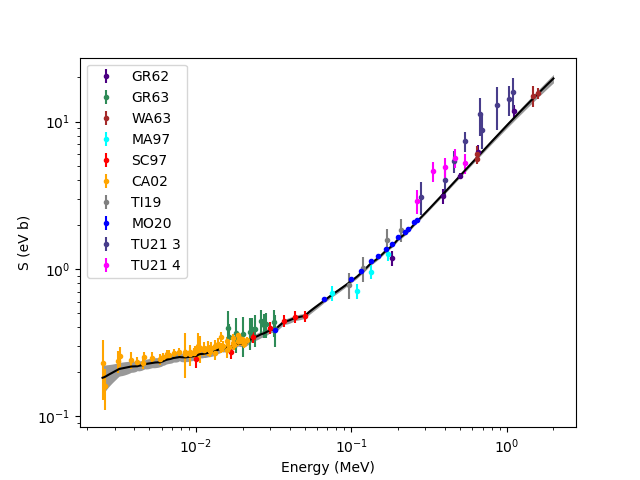
\includegraphics[width=\linewidth]{Figures/dphe3g_S.png}
    	\end{minipage}
    	\hspace{0mm}
    	\begin{minipage}{.48\textwidth}
        		\centering
        		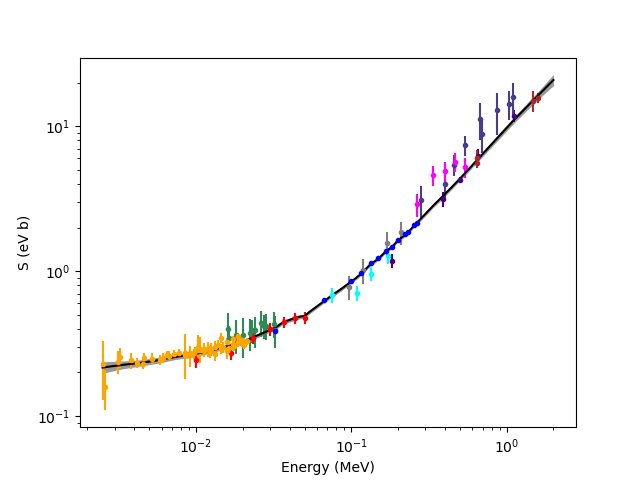
\includegraphics[width=\linewidth]{Figures/dphe3g_logS.png}
    	\end{minipage}
    	\begin{minipage}{.48\textwidth}
    		\centering
		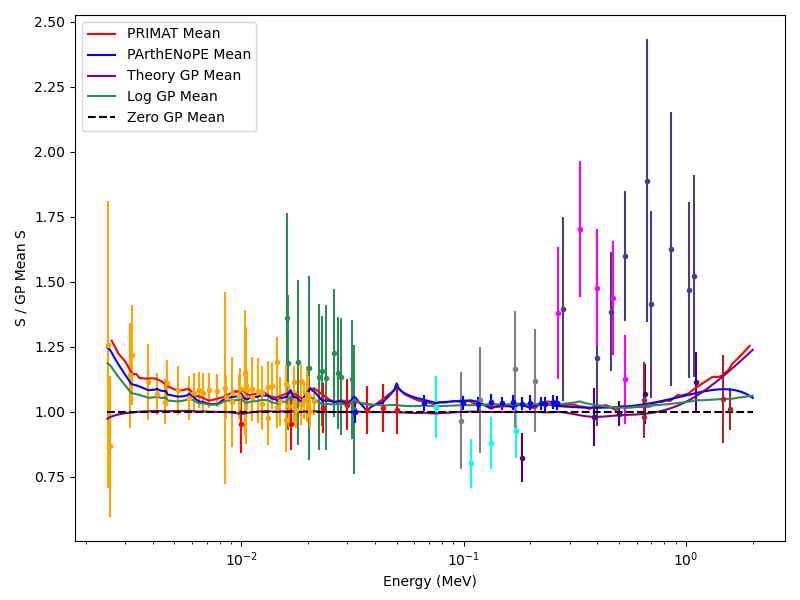
\includegraphics[width=\linewidth]{Figures/dphe3g_S_comp.png}	
	\end{minipage}
	\hspace{0mm}
	\begin{minipage}{.48\textwidth}
    		\centering
		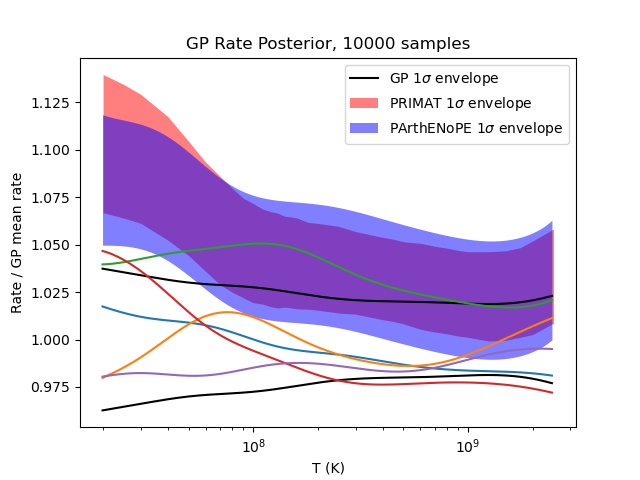
\includegraphics[width=\linewidth]{Figures/dphe3g_rate.png}	
	\end{minipage}
    	\caption{Gaussian process regression fits to $d$($p$,$\gamma$)$^3$He S-factor data. \textit{Top left}: Gaussian process mean and $1\sigma$ envelope in the BBN energy range. An uninformative zero mean prior and LDO hyperparameter optimization are used. The ten datasets \cite{Griffiths1962, Griffiths1963, Warren1963, Ma1997, Schmid1997, Casella2002, Mossa2020, Turkat2021} used to fit the model are shown with $1\sigma$ total error bars. \textit{Top right}: Gaussian process mean and $1\sigma$ envelope in the same energy range. This model is fit in $\log S$; the rest of the regression process is the same as in the top left plot. \textit{Bottom left}: In addition to the two models above, a Gaussian process fit to S-factor data (not $\log S$) with the theoretical calculation from \cite{Marcucci2016} as the prior mean. All three models, along with the best-fit S-factors from PRIMAT and PArthENoPE, are normalized to the Gaussian process mean in the top left plot. \textit{Bottom right}: Gaussian process S-factor fit in the top left plot integrated to get the reaction rate, along with the rates from PRIMAT and PArthENoPE. 5 samples drawn from the posterior are shown. }
\end{figure}

\begin{figure}
	\centering
	\begin{minipage}{0.48\textwidth}
		\centering
		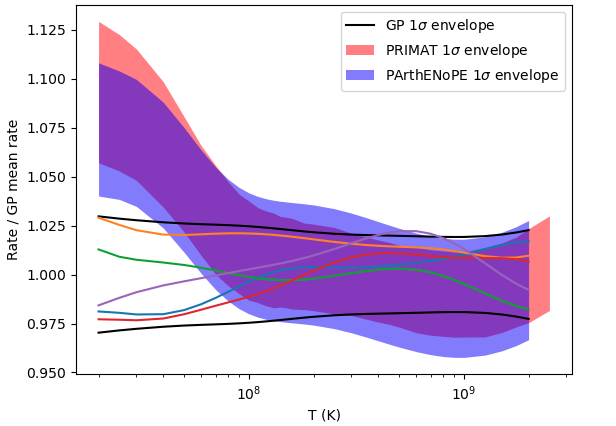
\includegraphics[width=\linewidth]{Figures/dphe3g_log_rate.png}
	\end{minipage}
	\hspace{0mm}
	\begin{minipage}{0.48\textwidth}
		\centering
		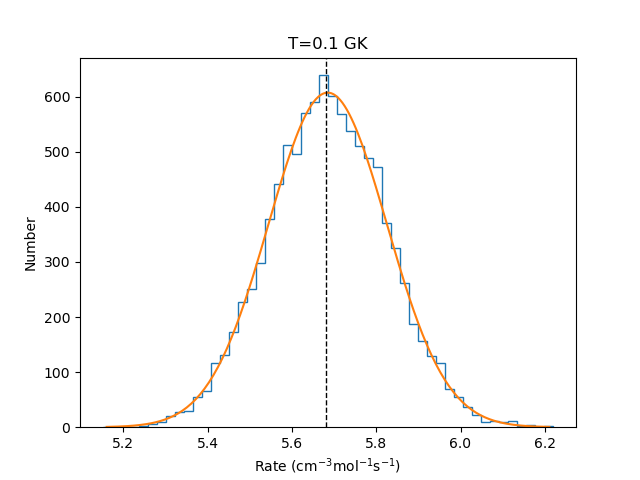
\includegraphics[width=\linewidth]{Figures/dphe3g_gaussian_rate.png}
	\end{minipage}
	\caption{$d$($p$,$\gamma$)$^3$He reaction rates for a Gaussian process fit to $\log S$ with a zero mean prior. \textit{Left}: The $1\sigma$ rate envelope, along with those of PRIMAT and PArthENoPE. 5 sample draws are shown. \textit{Right}: Histogram of the reaction rate at $10^8$ K, overlayed with a Gaussian fit. The black dashed line is the rate for the Gaussian process mean. }
\end{figure}

Figure 4 shows the reaction rate posterior for the Gaussian process fit to $\log S$. Above $10^8$ K the rate agrees significantly better with those of PRIMAT and PArthENoPE when compared to models fit directly to $S$. The rate remains $\gtrsim1\sigma$ discrepant at lower temperatures as the S-factor fit to the lowest energy LUNA data is still below other fits (see Figure 3). At each temperature, the rate posterior still follows a Gaussian distribution closely despite treating the S-factor as following a log-normal distribution, shown in the right plot. 

\subsection{Correlations}

\begin{figure}
	\begin{minipage}{.48\textwidth}
        		\centering
        		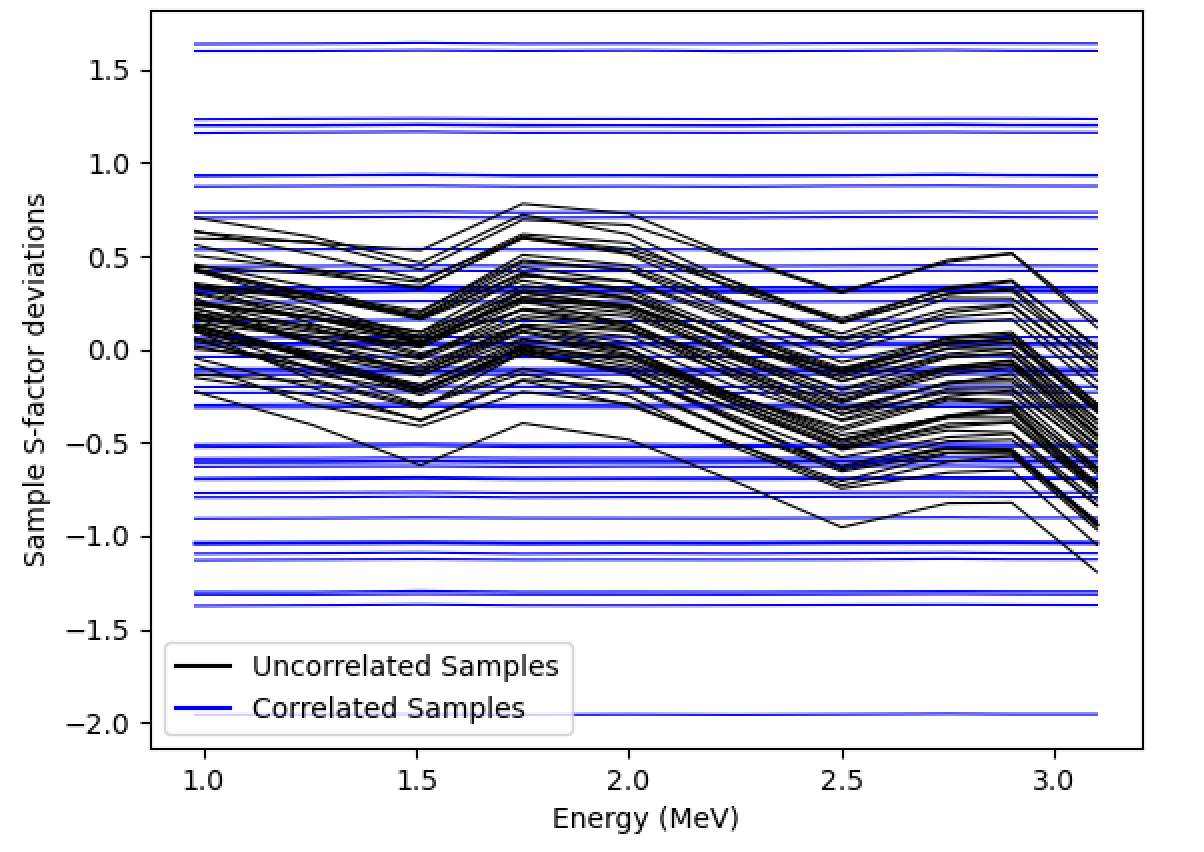
\includegraphics[width=\linewidth]{Figures/ddhe3n_correlations.png}
    	\end{minipage}
    	\hspace{0mm}
    	\begin{minipage}{.48\textwidth}
        		\centering
        		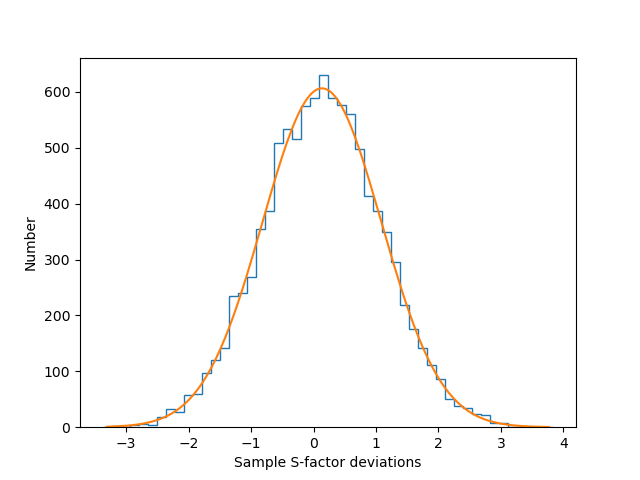
\includegraphics[width=\linewidth]{Figures/ddhe3n_correlation_hist.png}
    	\end{minipage}
	\caption{Sample draws from two Gaussian process posteriors, one including correlations and one excluding correlations. Zero mean priors and LDO hyperparameter optimization are used for both. \textit{Left}: 50 sample draws from both posteriors at the energies measured by SC72 \cite{Schulte1972} normalized to the reported values. \textit{Right}: Histogram of 10,000 samples from the correlated posterior showing the number of reported standard deviations at the lowest energy measured, overlayed with a Gaussian fit. }
\end{figure}

The S-factor plots normalized to the Gaussian process means shown in Figures 1 and 2 suggest that correlations are handled well by the Gaussian processes, since perfectly correlated data points lie the same percentage above or below the Gaussian process means. To further confirm that correlations are handled in a similar manner in individual S-factor samples, consider the high energy regime for $d$($d$,$n$)$^3$He. SC72 \cite{Schulte1972} collected data in this energy range with negligible statistical uncertainty, and so each point in this set is considered perfectly correlated with every other. If correlations are handled as expected, shifting each data point up or down by the same amount, then each sample draw should lie the same amount above or below the experimental data at the energies of those data points. 

Figure 5 shows sample draws at the SC72 energies from two Gaussian processes: one including correlations and one without. Every sample from the correlated posterior is the same distance from the reported values from SC72, while this is not true for the uncorrelated samples. At each energy, the mean of the samples is $0.13\sigma$ above the experimental mean, and the standard deviation of the samples is 95\% of the experimental standard deviation. The small differences here from 0 and 1 respectively are from the influence of lower energy data on the Gaussian process fit. This result confirms that the correlations are handled robustly by Gaussian processes. 



\section{Primordial Abundances}


To propagate reported uncertainties in experimental S-factor data to uncertainties in primordial abundance predictions, samples drawn from Gaussian process posteriors are passed into a slightly modified version of LINX that allows for custom rates to be used for as many of the 12 key reactions as desired. For each sample, the final abundances of hydrogen, deuterium, helium-3, and helium-4 are recorded. Reported central values and error bars are the mean and standard deviation for each abundance, always closely following a Gaussian distribution. 10,000 samples are used for every reaction combination, hyperparameter optimization method, and kernel choice considered. When multiple reactions are varied simultaneously, they are considered uncorrelated\footnote{Acknowledgement of this assumption is important as theoretical predictions suggest that the two $d$+$d$ reactions are not independent of one another, but handling this in a more sophisticated manner is well beyond the scope of this work.}. 

Each prediction is compared with those from exclusively using the rates from PRIMAT and PArthENoPE. Error bars for these depend on which Gaussian process rates are varied. Without the Gaussian process framework for drawing samples, uncertainties for these rates are estimated by modeling them as following a log-normal distribution
\begin{equation}
	\log R(T) = \log \bar{R}(T) + q \log \Delta R(T), \nonumber
\end{equation}
where $\bar{R}(T)$ and $\Delta R(T)$ are the mean and $1\sigma$ rates at temperature $T$ and $q\sim\mathcal{N}(0,1)$. When only a single rate is varied, the error bars reported below for the PRIMAT and PArthENoPE rates are simply obtained by calculating the abundances for $q=0$ and $q=1$. When multiple rates are varied, $q$ is sampled for each rate 10,000 times and used in LINX. The error bars for PRIMAT and PArthENoPE rates are therefore larger when more rates are considered. 

The subsections below walk through the impact on predicted abundances when Gaussian process regression is used for each reaction combination. Generally, using theoretical instead of zero mean priors makes very little difference, and using marginal likelihood instead of LDO hyperparameter optimization has a larger, yet still small, impact. Each reaction agrees quite well with the PRIMAT result, and when the deuterium burning rates are combined, the predicted deuterium abundances are within $0.15\sigma$ with roughly similar uncertainties.

\subsection{d(d,n)$^3$He}

\begin{figure}
	\centering
	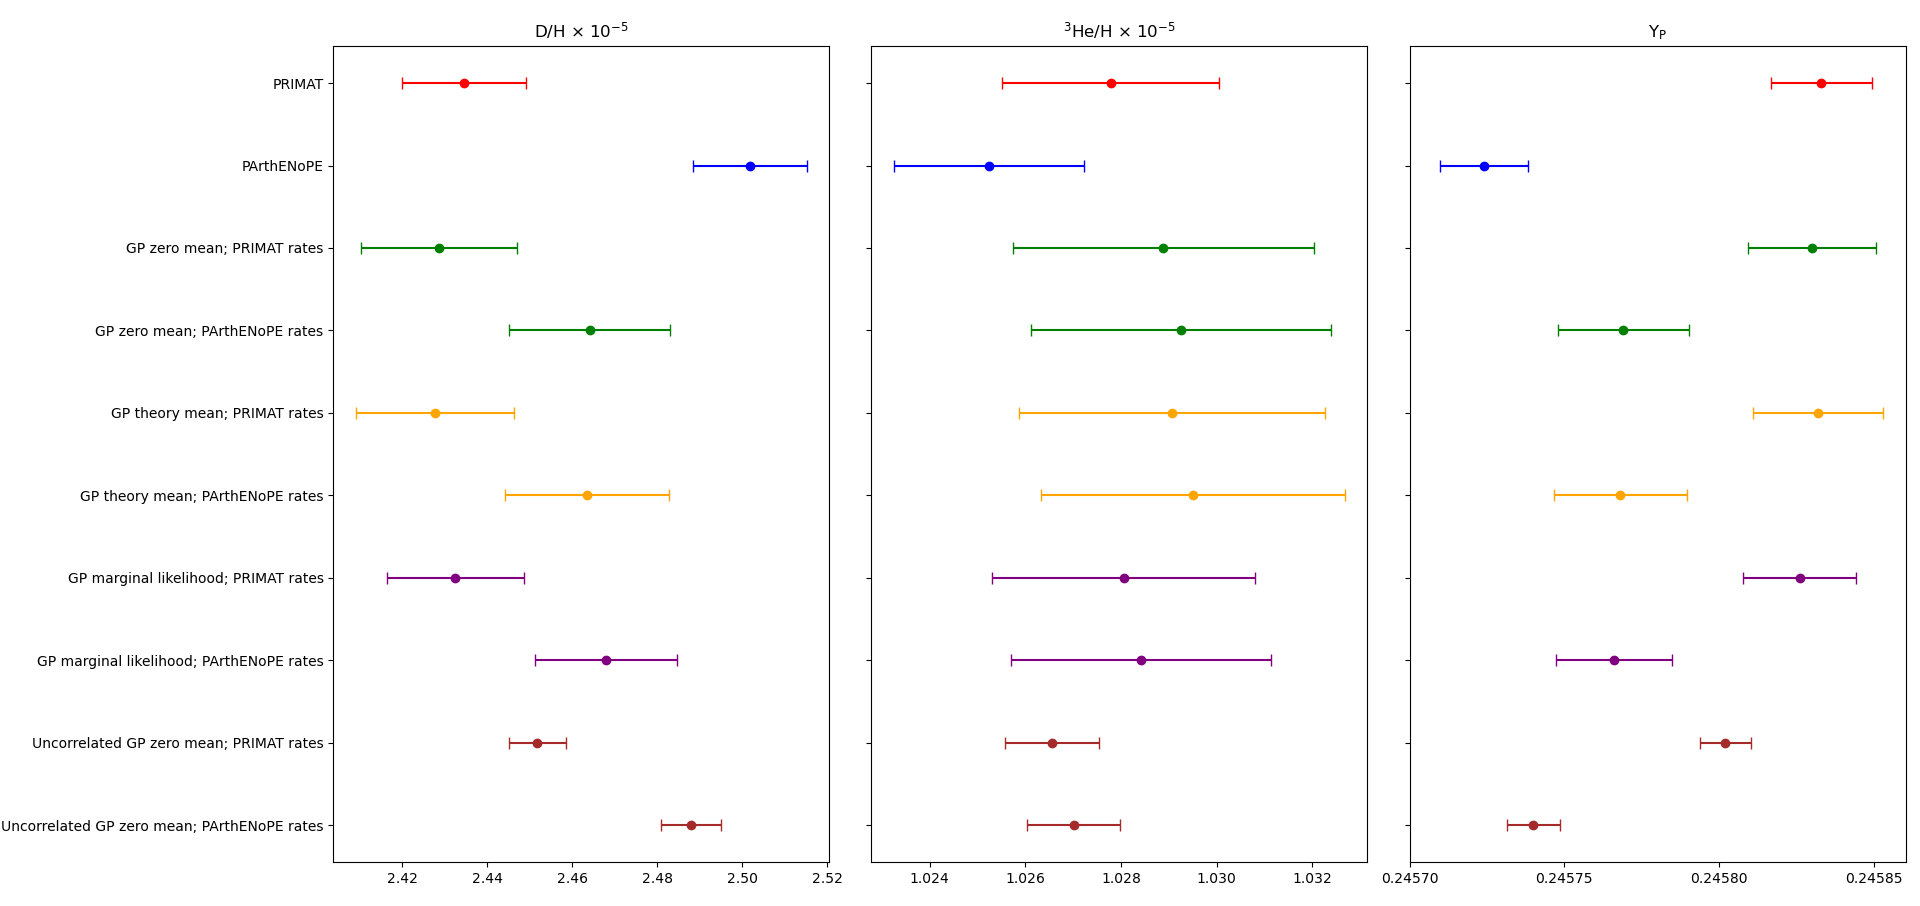
\includegraphics[width=0.98\linewidth]{Figures/ddhe3n_comp.png}
	\caption{Comparison of primordial abundance predictions using Gaussian process regression to fit $d$($d$,$n$)$^3$He data. Unless otherwise specified, LDO optimization is used for hyperparameter selection and correlations are fully included during regression. Results from using exclusively rates from PRIMAT and PArthENoPE are also shown. }
\end{figure}

Figure 6 shows D/H, $^3$He/H, and Y$_\text{P}$ predictions when using four different Gaussian process fits to $d$($d$,$n$)$^3$He: a zero mean prior and theory mean prior using LDO optimization, a zero mean prior using marginal likelihood optimization, and a zero mean prior using LDO optimization without the inclusion of correlations. For each Gaussian process fit, both PRIMAT and PArthENoPE networks are used for the other rates, giving eight sets of predictions in total. Table 1 in section 8 contains the numerical values shown in this figure. The uncorrelated Gaussian process produces uncertainties much smaller than the other scenarios, as expected with more degrees of freedom during regression. The theory mean prior makes minimal difference on abundance predictions. Uncertainties for the two LDO cases are around 25\% larger than PRIMAT and PArthENoPE. Using marginal likelihood optimization changes abundances by $\sim0.25\sigma$ and shrinks uncertainties by around 10\%. These observations apply both when PRIMAT and PArthENoPE networks are used for the other rates. 

The predicted deuterium abundance with the PRIMAT network\footnote{This whole comparison feels super clunky, but I am not sure how best to explain otherwise. } decreases slightly with the Gaussian process The decrease with the PArthENoPE network is much more significant, with the predicted value lying between the predictions from using exclusively the PRIMAT and PArthENoPE networks. One would expect predicted helium-3 abundances to therefore increase, since more deuterium is converted to helium-3 with the Gaussian process rate; this is reflected in the abundance results. The predicted helium-3 abundance is higher when the PArthENoPE network is used from other relevant reactions, despite the base PArthENoPE calculation having the lowest predicted helium-3 abundance. The helium-4 abundance remains relatively similar using the PRIMAT network and increases when using the PArthENoPE network. 

\subsection{d(d,p)t}

\begin{figure}
	\centering
	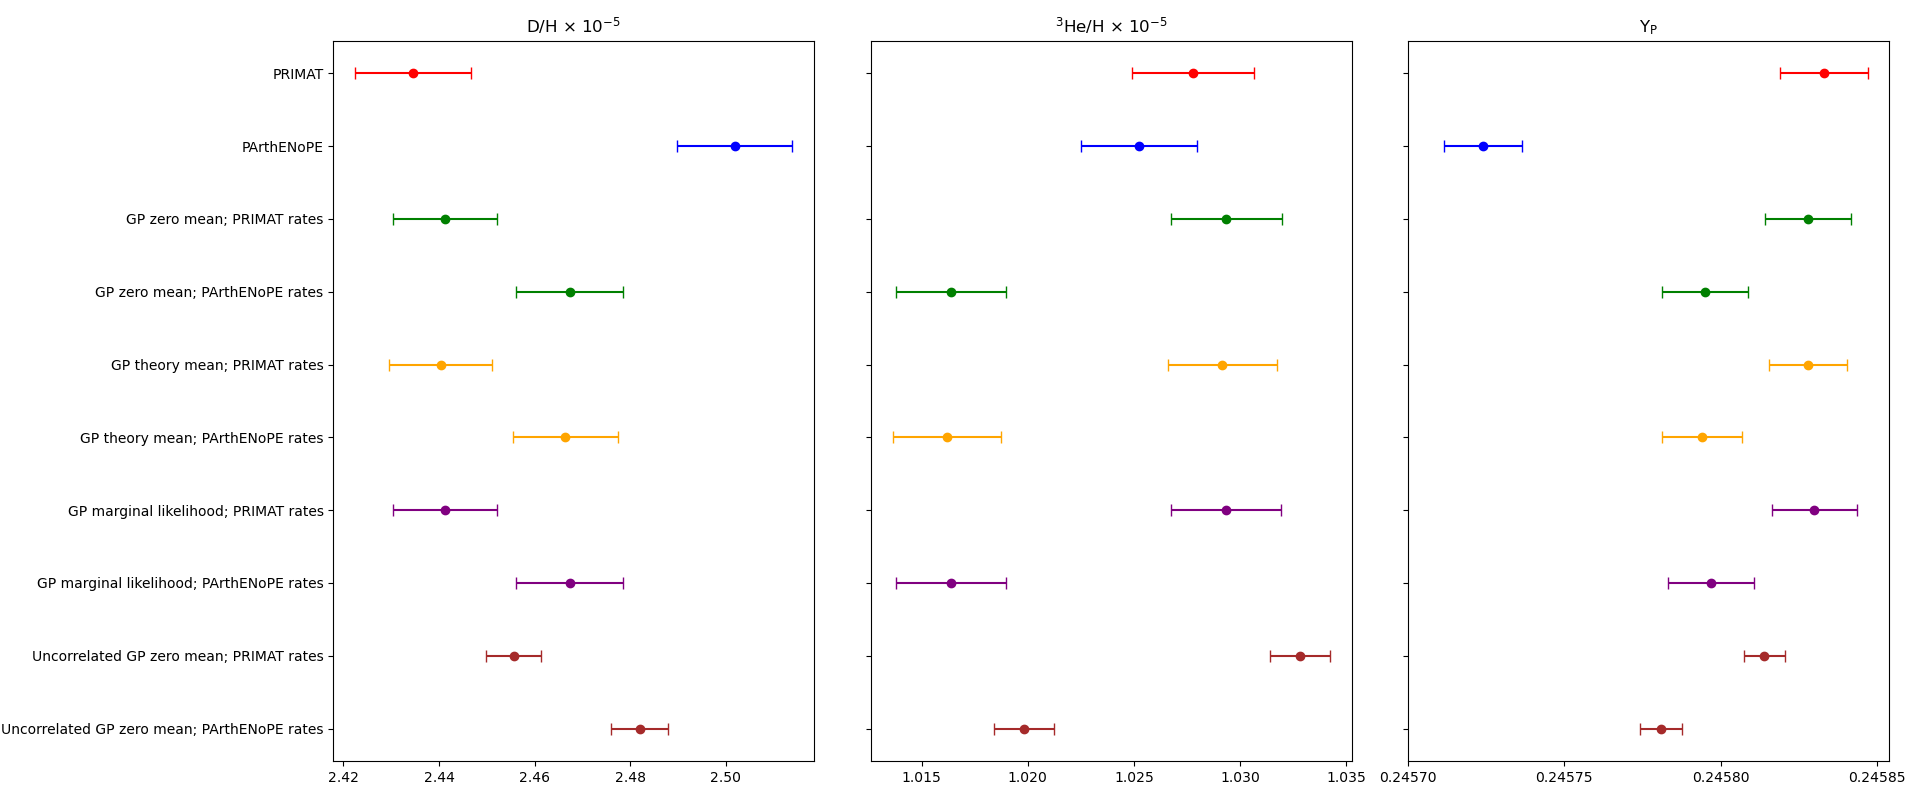
\includegraphics[width=0.98\linewidth]{Figures/ddtp_comp.png}
	\caption{Comparison of primordial abundance predictions using Gaussian process regression to fit $d$($d$,$p$)$t$ data. Unless otherwise specified, LDO optimization is used for hyperparameter selection and correlations are fully included during regression. Results from using exclusively rates from PRIMAT and PArthENoPE are also shown.}
\end{figure}

Figure 7 shows D/H, $^3$He/H, and Y$_\text{P}$ predictions when using different Gaussian process fits to $d$($d$,$p$)$t$. Table 2 in section 8 contains the numerical values shown in this figure. Again, uncertainties with the uncorrelated Gaussian process are smaller than all other cases, and a theory mean prior makes minimal difference in abundances. Marginal likelihood optimization yields nearly identical results as LDO optimization for this reaction. Unlike $d$($d$,$n$)$^3$He, uncertainties shrink by around 10\% when the Gaussian process rates are used.

The predicted deuterium abundance with the PRIMAT network increases slightly with the Gaussian process. Again, the deuterium abundance with the PArthENoPE network decreases significantly with the Gaussian process, with the predicted value lying between the predictions from using only PRIMAT and PArthENoPE rates. The predicted helium-3 abundance now is lower when the PArthENoPE network is used from other relevant reactions. The helium-4 abundance remains relatively similar using the PRIMAT network and increases when using the PArthENoPE network; this increase is greater than with $d$($d$,$n$)$^3$He. 

\subsection{d+d Rates}

\begin{figure}
	\centering
	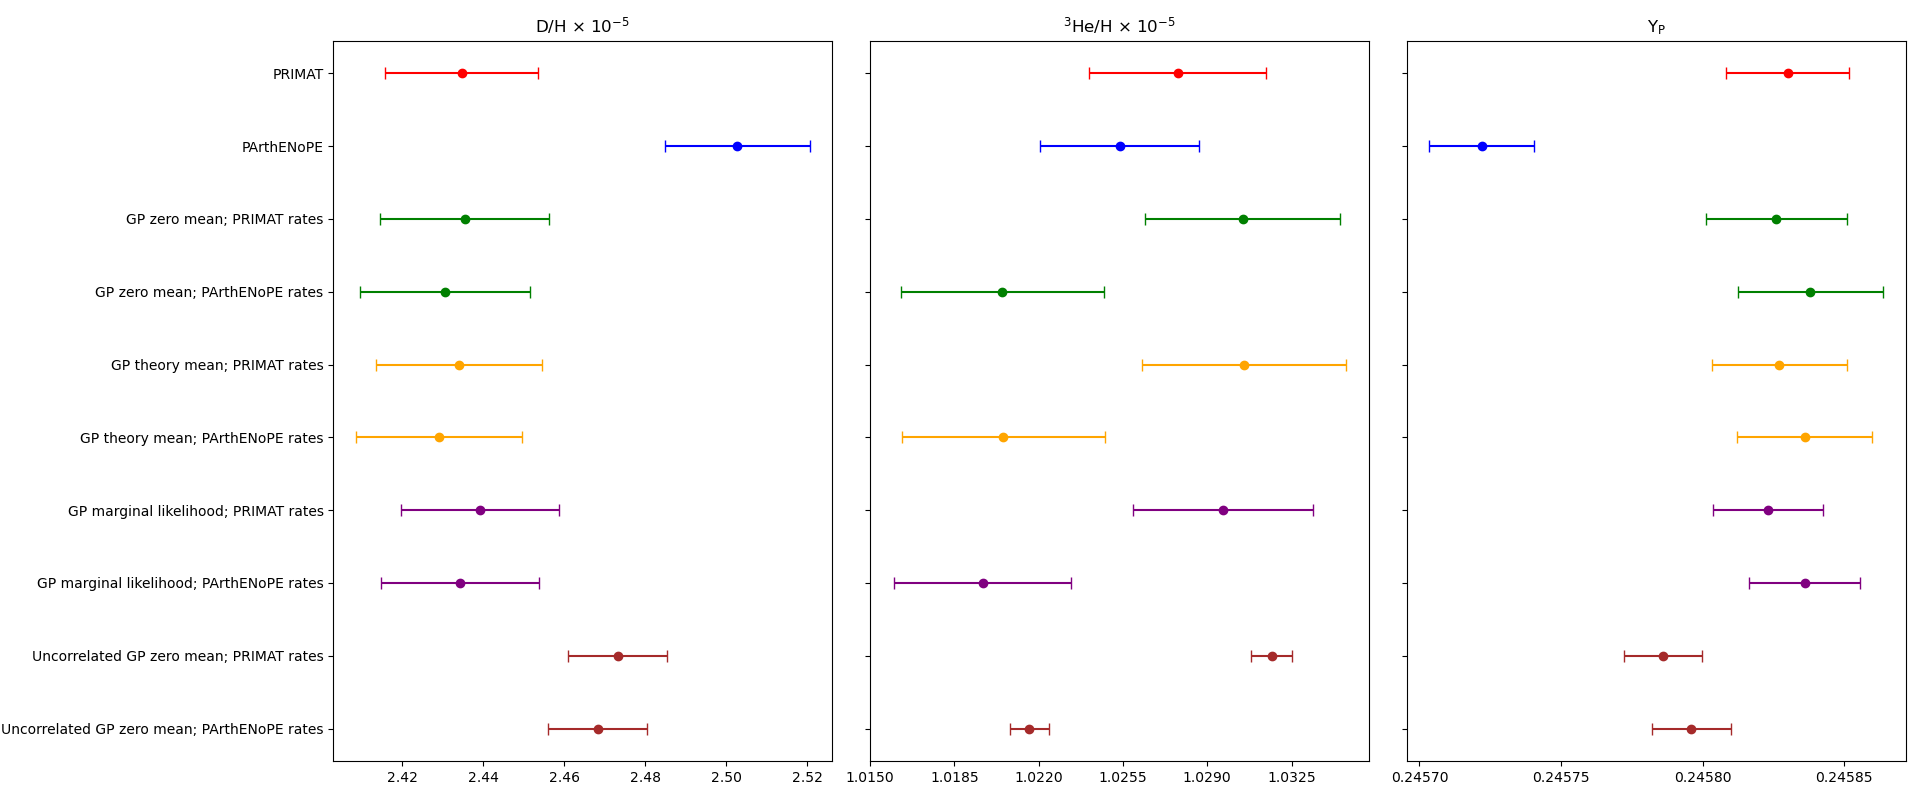
\includegraphics[width=0.98\linewidth]{Figures/dd_comp.png}
	\caption{Comparison of primordial abundance predictions using Gaussian process regression to fit both $d$($d$,$n$)$^3$He and $d$($d$,$p$)$t$ data. Unless otherwise specified, LDO hyperparameter optimization is used and correlations are fully included during regression. Results from using exclusively rates from PRIMAT and PArthENoPE are also shown.}
\end{figure}

Figure 8 shows D/H, $^3$He/H, and Y$_\text{P}$ predictions when using different Gaussian process fits to $d$($d$,$n$)$^3$He and $d$($d$,$p$)$t$ simultaneously. Table 3 in section 8 contains the numerical values in this figure. As expected from varying these rates individually, uncertainties with the uncorrelated Gaussian process are smaller than all other cases, and a theory mean prior makes minimal difference in abundances. Since marginal likelihood optimization shifts central values by around 25\% for $d$($d$,$n$)$^3$He alone and has negligible impact for $d$($d$,$p$)$t$, the 25\% shift remains for this combination. Again, uncertainties slightly decrease with marginal likelihood optimization.

Predicted deuterium abundances now agree well with the base PRIMAT calculation when either PRIMAT or PArthENoPE networks are used along with the Gaussian processes; this makes sense as two of the three most relevant reactions for deuterium production are the same, and the third is very similar in both networks. $d$($d$,$n$)$^3$He shifts the deuterium abundance down while $d$($d$,$p$)$t$ shifts it back up, creating the best agreement when combined. Helium-3 abundances become more discrepant due to the other relevant reactions, with abundances from the PRIMAT network slightly higher than the base PRIMAT calculation (from $d$($d$,$n$)$^3$He) and those using the PArthENoPE network lower. The helium-4 abundances all remain close to the PRIMAT calculation even when using the PArthENoPE network for the other rates. 

\begin{figure}
	\centering
	\begin{minipage}{0.32\textwidth}
		\centering
		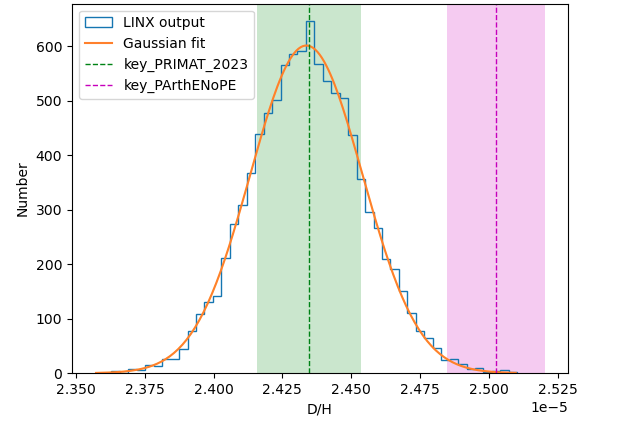
\includegraphics[width=\linewidth]{Figures/dd_theory_dh.png}
	\end{minipage}
	\hspace{0mm}
	\begin{minipage}{0.32\textwidth}
		\centering
		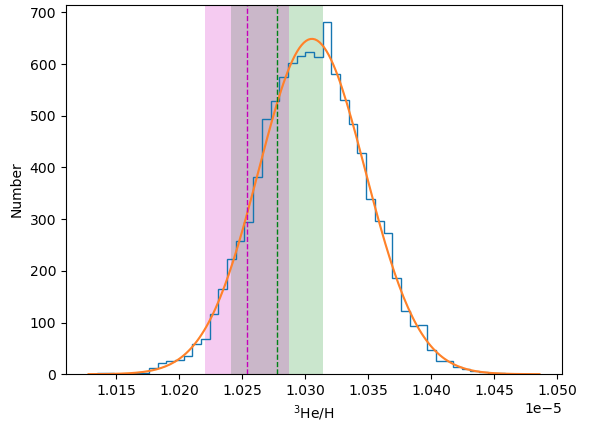
\includegraphics[width=\linewidth]{Figures/dd_theory_he3h.png}
	\end{minipage}
	\hspace{0mm}
	\begin{minipage}{0.32\textwidth}
		\centering
		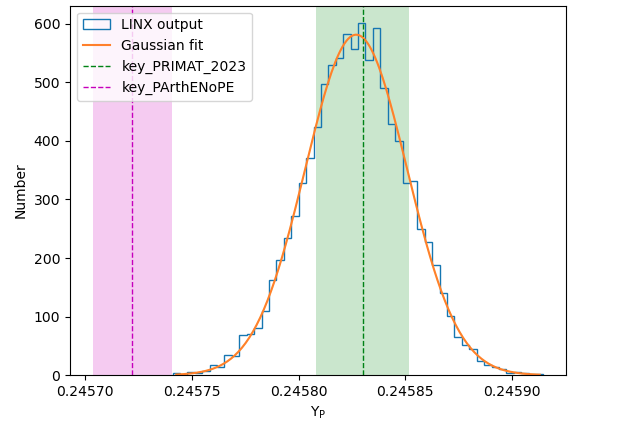
\includegraphics[width=\linewidth]{Figures/dd_theory_yp.png}
	\end{minipage}
	\caption{Histograms of primordial abundance predictions using Gaussian process regression to fit both $d$($d$,$n$)$^3$He and $d$($d$,$p$)$t$ data. 10,000 samples are shown. A Gaussian fit is overlayed on each, and $1\sigma$ envelopes for PRIMAT and PArthENoPE are shown as vertical bands.}
\end{figure}

Figure 9 shows histograms for D/H, $^3$He/H, and Y$_\text{P}$ predictions using Gaussian processes fit with theory mean priors for $d$($d$,$n$)$^3$He and $d$($d$,$p$)$t$ and the PRIMAT network for other reactions. A Gaussian fit is overlayed on each; all three distributions closely follow Gaussian distributions. The $1\sigma$ envelopes of PRIMAT and PArthENoPE are shown as vertical bands on each plot. 

\subsection{d(p,$\gamma$)$^3$He}

\begin{figure}
	\centering
	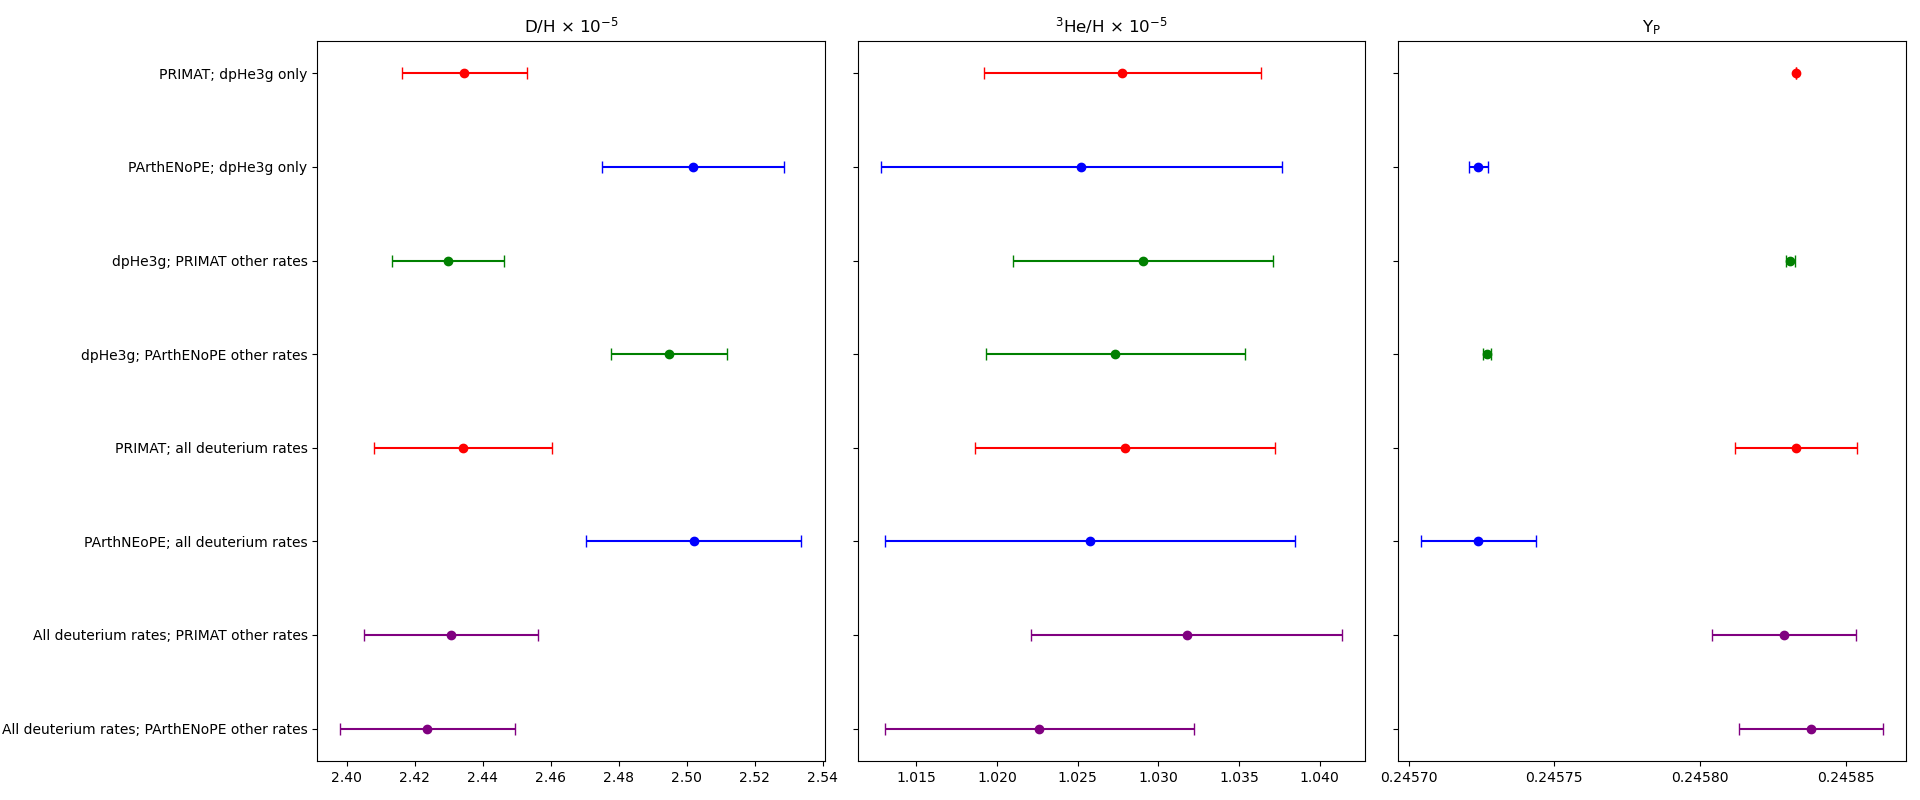
\includegraphics[width=0.98\linewidth]{Figures/dphe3g_comp.png}
	\caption{Comparison of primordial abundance predictions using Gaussian process regression to fit $d$($p$,$\gamma$)$^3$He data in $\log S$. The top four points vary only this reaction, while the bottom four also vary $d$($d$,$n$)$^3$He and $d$($d$,$p$)$t$. For each reaction, LDO hyperparameter optimization and a zero mean prior are used for regression. }
\end{figure}

Figure 10 shows D/H, $^3$He/H, and Y$_\text{P}$ predictions using the Gaussian process fit to $d$($p$,$\gamma$)$^3$He in $\log S$, with a zero mean prior and LDO hyperparameter optimization. The top four points use only this reaction, and the bottom four in addition use the zero mean prior, LDO optimized Gaussian process fits to $d$($d$,$n$)$^3$He and $d$($d$,$p$)$t$. Table 4 in section 8 contains the numerical values in this figure. When varying only $d$($p$,$\gamma$)$^3$He, uncertainties for D/H and $^3$He/H are smaller than with PRIMAT and PArthENoPE. Deuterium central values with both networks decrease slightly, and helium-3 central values increase; the Gaussian process rate is slightly higher between 0.3 and 2 GK, so this result is expected. The much lower rate at temperatures below 0.1 GK predicted by Gaussian process regression does not matter for these calculations. Small shifts in Y$_\text{P}$ are due to changes in deuterium and helium-3 propagating to other reactions, as this reaction has little direct impact on helium-4. 

When all three deuterium burning reactions are sampled from Gaussian processes, there is remarkable agreement with the calculation of PRIMAT for D/H and Y$_\text{P}$ both in central values and uncertainties. Uncertainties on helium-3 are dominated by $d$($p$,$\gamma$)$^3$He; therefore, all predictions roughly agree. 



\section{Future Work}



There are a few outstanding questions for this technique, but they are (for now) left for future work. It would be interesting to apply Gaussian process regression to the other nine key reactions to analyze impacts on lithium and helium-3, particularly $^3$He($d$,$p$)$\alpha$; the rates from PRIMAT and PArthENoPE disagree by multiple $\sigma$ toward the low temperature range for BBN. Additionally, this reaction contains a broad resonance, and it would be interesting to check whether the Gaussian process approach can model resonances as well. 

Cosmological parameter estimation becomes more difficult with Gaussian processes; there are now infinitely many nuisance parameters to marginalize over instead of just one per reaction. The trained Gaussian processes provide priors for estimation; one could imagine performing sampling without treating these as nuisance parameters, drawing sample functions at each step, or choosing some pivot energies and marginalizing over the S-factor at those energies. 

It would be fantastic to inject mock datasets to estimate to what extent uncertainties can be reduced from future experiments. If a new dataset could be generated with uncertainties that are reasonable given current experimental capabilities, it would be simple to add to the Gaussian process pipeline. It is still unclear how such a mock dataset should be created\footnote{It is probably a good idea to talk to a nuclear experimentalist about how to do this}. 

Kernel hyperparameter marginalization is, and will most likely always, be left for future work. However, considering marginal likelihood optimization in addition to LDO optimization helps to provide some sense of the sensitivity of results to hyperparameter choice. In both cases, the general trends are the same (with some details differing). 



\section{Gaussian Processes}



A Gaussian process is a stochastic process in which a collection of random variables jointly follow a multivariate normal distribution \cite{Rasmussen2006}. To use a Gaussian process here, the experimentally measured S-factor values are assumed to be drawn from the same latent function (the ``true'' S-factor) with Gaussian noise. By discretizing the relevant energy range, the probability distribution of the latent function can be modeled as following a multivariate normal distribution with some mean and covariance matrix.

For a given reaction, let $S$ and $S_*$ denote the measured S-factor values and latent function values (to be inferred) respectively. In subsequent equations, these quantities are vectors. The partitioned multivariate normal distribution is 
\begin{equation}
	\begin{bmatrix}
   		S \\ S_*
	\end{bmatrix} \sim \mathcal{N} \left( 
	\begin{bmatrix}
    		\mu \\ \mu_*
	\end{bmatrix} , \begin{bmatrix}
    		K_{11} & K_{12} \\ K_{21} & K_{22}
	\end{bmatrix} \right),
\end{equation}
where $\mu$ is the function mean prior and $K$ describes the correlation between points in input space. The predictive mean and covariance for the underlying function are \cite{Rasmussen2006}
\begin{equation}
	\mu_{S_* | S} = \mu_* + K_{21} K_{11}^{-1}(S - \mu), \quad \Sigma_{S_* | S} = K_{22} - K_{21} K_{11}^{-1} K_{12}.
\end{equation}
$\mu$ is often set to zero for a purely data-driven approach since the predictive mean is non-zero; however, prior information (in this case, theoretical calculations) can be included in $\mu$. The kernel is a function of two points in input space that encodes the correlation between the latent function values at those points. Kernels also include other hyperparameters $\theta$ that must be chosen. Selecting the functional form of the kernel is a key part of using Gaussian processes for regression and should be chosen by considering the properties that the underlying function is expected to follow. Kernels can be added or multiplied (including by an overall constant) and remain a valid kernel. 

In (3), $K_{12}$, $K_{21}$ and $K_{22}$ are entirely set by the kernel. For the selected kernel $k$, the $ij^{th}$ component of $K_{12}$ is given by
\begin{equation}
	K_{12,ij} = k(E_i, E_{*j}), \nonumber
\end{equation}
where $E_i$ is the energy for the $i^{th}$ entry in the vector of S-factor measurements $S$ and $E_{*j}$ is the $j^{th}$ entry in the vector of energies at which to make predictions. Similarly, the $ij^{th}$ component of $K_{22}$ is given by
\begin{equation}
	K_{22,ij} = k(E_{*i}, E_{*j}). \nonumber
\end{equation}
$K_{11}$ can also be entirely set by the kernel, or known variance in the data can be included in addition. This allows both statistical and systematic errors as reported for each dataset to be included as a full covariance matrix $\Sigma$ that is added to the kernel component, modeling both correlations from experiments and correlations from the latent function. The $ij^{th}$ component of $\Sigma$, where point $i$ is from dataset $k$ and point $j$ is from dataset $l$ is given by
\begin{equation}
	\Sigma_{i_k j_l} = \delta_{ij} \sigma_{stat,i} \sigma_{stat,j} + \delta_{kl} \sigma_{sys,i} \sigma_{sys,j}. \nonumber
\end{equation}

After selecting a particular kernel, the hyperparameters must be chosen in a principled manner before using (4) to draw samples from the posterior. One of the most common ways to do this is to maximize the marginal likelihood of observing the known data given a particular choice of hyperparameters, or equivalently minimizing the negative log likelihood: 
\begin{equation}
	-\log{p\left( S | \vec{\theta} \right)} = \frac{1}{2} \left( S^T K_{11}^{-1} S + \log{|K_{11}|} + n \log{2\pi} \right).
\end{equation}
where $n$ is the number of data points \cite{Rasmussen2006}. Cross-validation, where a subset of the training data is left out from the rest of the set and the probability of observing those points given the remaining data is maximized, directly evaluates the model's performance on energy regions without known data. For this application, an individual dataset is left out from the rest. The model makes predictions using (4) at those energies and compares them to the experimental values. For a set of hyperparameters $\theta$, each dataset is left out one at a time, and the sum of the log likelihoods is used to evaluate the model's performance before updating the hyperparameters:
\begin{equation}
	\mathcal{L}_{LDO} = \sum_{i\in\text{sets}} \log p(S_i | S_{-i}),
\end{equation}
where $S_i$ and $S_{-i}$ denote the S-factor measurements in dataset $i$ and all other datasets respectively. The log likelihood to observe dataset $i$ given the other datasets is 
\begin{equation}
	\log p(S_i | S_{-i}) = -\frac{1}{2} \left( (S_i - \mu_{S_i | S_{-i}})^T \Sigma_{S_i | S_{-i}}^{-1} (S_i - \mu_{S_i | S_{-i}}) + \log \det  \Sigma_{S_i | S_{-i}} + n_i \log 2\pi \right), \nonumber
\end{equation}
where $\mu_{S_i | S_{-i}}$ is the conditional mean from (4),  $\Sigma_{S_i | S_{-i}}$ is the conditional covariance matrix from (4), and $n_i$ is the number of datapoints in dataset $i$. This ``Leave-Dataset-Out'' (LDO) likelihood is maximized for most hyperparameter selections in this work. Reasonable kernel choices considered have the flexibility (with very small correlation lengths) to perfectly fit through every data point. Using the ``Leave-One-Out'' cross-validation method, a common choice for cross-validation, leads to extreme overfitting during hyperparameter selection. This problem can either be solved by placing a highly-informative, somewhat arbitrarily-chosen prior for the correlation lengths, or by utilizing the LDO likelihood. Uninformative uniform priors are placed on the hyperparameters when either (5) or (6) are used.

With at most four hyperparameters for any given kernel used here, methods such as an MCMC or simulated annealing to optimize the likelihood are not necessary, and gradient descent is preferred. To avoid convergence to local minima in hyperparameter space, using a gradient descent algorithm that incorporates momentum when updating hyperparameters, in this case the \textit{Adam} optimizer, is very helpful, as either likelihood choice is not generally convex. The code\footnote{It is simple to modify the default code provided by scikit-learn to add off-diagonal terms to $\Sigma$, but very challenging to implement hyperpriors and custom gradient descent algorithms. On the other hand, it is straightforward to have custom hyperpriors and gradient descent algorithms using the default code from PyTorch, but very challenging to add off-diagonal terms to $\Sigma$ within their framework. \phantom{Some text to help with formatting.}} used for all Gaussian process regression tasks in this project, fully implemented in JAX, can be found \href{https://github.com/tim-launders/bbn_gaussian_processes}{here}.



\section{Kernel Selection}



An important test for this method is to consider sensitivity to kernel choice and determine which kernels are ``valid'' for this analysis. As mentioned previously, kernel choices must include components to capture large scale correlations and small scale fluctuations. The first of these can be done with a large-$\nu$ Mat\'ern or squared exponential; the second with a small-$\nu$ Mat\'ern. Figure 9 shows D/H, $^3$He/H, and Y$_\text{P}$ predictions when using various kernels that fit these criteria to fit $d$($d$,$n$)$^3$He using a zero prior mean. Additionally, a simpler case using only a Mat\'ern-1/2 kernel is considered, which leads to a ``worse'' fit overall. Decreasing the large correlation $\nu$ slightly lowers final deuterium abundances. Raising the smaller $\nu$ has a more significant effect, decreasing predicted deuterium abundances while increasing the error bars. The kernel combination of squared exponential with Mat\'ern-1/4 is selected for further analyses, giving fit shapes with the least deviation from other fits\footnote{We know, for example, that in the energy range without data points, samples should not dip very low before reaching the high energy dataset}. Overall, this decision\footnote{May want to select different kernels for this comparison, or only show fewer choices} affects predicted abundances by much less than $1\sigma$.

\begin{figure}
	\centering
	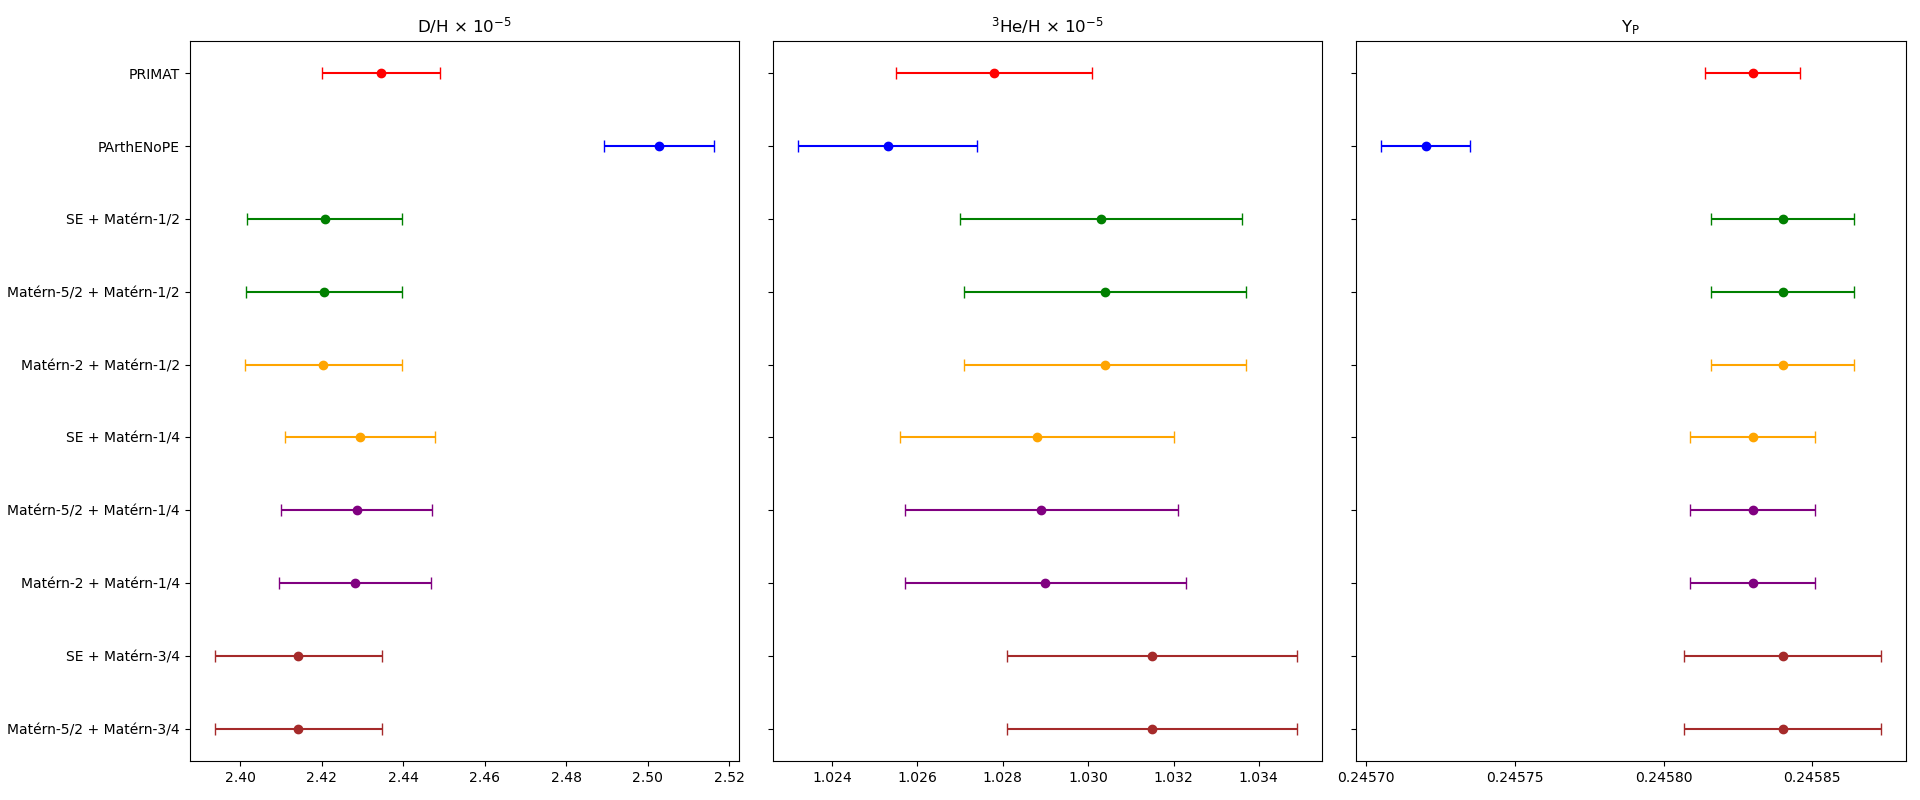
\includegraphics[width=0.98\linewidth]{Figures/ddhe3n_kernel_comp.png}
	\caption{Comparison primordial abundance predictions for different kernels used to perform Gaussian process regression on $d$($d$,$n$)$^3$He S-factor data.  For all kernel choices, a zero prior mean and LDO hyperparameter selection are used. The key\_PRIMAT\_2023 network is used for all other reactions. All error bars represent $1\sigma$ uncertainties from 10,000 samples drawn from the posteriors. \textit{Left}: D/H predictions for different kernels. \textit{Middle}: $^3$He/H predictions for different kernels. \textit{Right}: Y$_\text{P}$ predictions for different kernels. }
\end{figure}



\section{Dataset Selection}



This section will discuss which experimental data sets are chosen for each deuterium burning reaction and why. 

\subsection{d(d,n)$^3$He}

\subsection{d(d,p)t}

\subsection{d(p,$\gamma$)$^3$He}


\section{Primordial Abundance Tables}



\begin{table*}[ht]
    \centering
    \caption{Comparison of primordial abundance predictions using Gaussian process regression to fit $d$($d$,$n$)$^3$He data. Unless otherwise specified, LDO is used for hyperparameter optimization and correlations are fully included during regression. Companion table for Figure 6.}
    \small
    \begin{tabular}{l
                    S[table-format=1.6]
                    S[table-format=1.5]
                    S[table-format=1.3]
                    S[table-format=1.6]
                    S[table-format=1.5]
                    S[table-format=1.3]
                    S[table-format=1.6]
                    S[table-format=1.7]
                    S[table-format=1.4]} 
     \toprule
    {Model} & {D/H × $10^{-5}$\,} & {\,D/H $1\sigma$ \%\,} &
    {\,$^3$He/H × $10^{-5}$\,} & {\,$^3$He/H $1\sigma$ \%\,} &
    {\,Y$_\text{P}$\,} & {\,Y$_\text{P}\,$ $\,1\sigma$ \%} \\
    \midrule
    PRIMAT & 2.435 & 0.60 & 1.0278 & 0.22 & 0.245833 & 0.0067 \\
    PArthENoPE & 2.502 & 0.53 & 1.0252 & 0.19 & 0.245724 & 0.0058 \\
    Zero mean; PRIMAT rates & 2.429 & 0.75 & 1.0289 & 0.31 & 0.245830 & 0.0084 \\
    Zero mean; PArthENoPE rates & 2.464 & 0.77 & 1.0292 & 0.30 & 0.245769 & 0.0086 \\
    Theory mean; PRIMAT rates & 2.428 & 0.77 & 1.0291 & 0.31 & 0.245832 & 0.0085 \\
    Theory mean; PArthENoPE rates & 2.464 & 0.78 & 1.0295 & 0.31 & 0.245768 & 0.0088 \\
    Marginal likelihood; PRIMAT rates & 2.432 & 0.66 & 1.0281 & 0.27 & 0.245826 & 0.0074 \\
    Marginal likelihood; PArthENoPE rates & 2.468 & 0.68 & 1.0284 & 0.27 & 0.245766 & 0.0076 \\
    Uncorrelated; PRIMAT rates & 2.452 & 0.28 & 1.0266 & 0.10 & 0.245802 & 0.0034 \\
    Uncorrelated; PArthENoPE rates & 2.488 & 0.28 & 1.0270 & 0.10 & 0.245740 & 0.0035 \\
    \bottomrule
    \end{tabular}
\end{table*}

\begin{table*}[ht]
    \centering
    \caption{Comparison of primordial abundance predictions using Gaussian process regression to fit $d$($d$,$p$)$t$ data. Unless otherwise specified, LDO is used for hyperparameter optimization and correlations are fully included during regression. Companion table for Figure 7.}
    \small
    \begin{tabular}{l
                    S[table-format=1.6]
                    S[table-format=1.5]
                    S[table-format=1.3]
                    S[table-format=1.6]
                    S[table-format=1.5]
                    S[table-format=1.3]
                    S[table-format=1.6]
                    S[table-format=1.7]
                    S[table-format=1.4]} 
     \toprule
    {Model} & {D/H × $10^{-5}$\,} & {\,D/H $1\sigma$ \%\,} &
    {\,$^3$He/H × $10^{-5}$\,} & {\,$^3$He/H $1\sigma$ \%\,} &
    {\,Y$_\text{P}$\,} & {\,Y$_\text{P}\,$ $\,1\sigma$ \%} \\
    \midrule
    PRIMAT & 2.435 & 0.50 & 1.0278 & 0.28 & 0.245833 & 0.0060 \\
    PArthENoPE & 2.502 & 0.48 & 1.0252 & 0.27 & 0.245724 & 0.0050 \\
    Zero mean; PRIMAT rates & 2.441 & 0.45 & 1.0294 & 0.25 & 0.245828 & 0.0060 \\
    Zero mean; PArthENoPE rates & 2.467 & 0.45 & 1.0164 & 0.25 & 0.245795 & 0.0060 \\
    Theory mean; PRIMAT rates & 2.440 & 0.44 & 1.0292 & 0.25 & 0.245828 & 0.0050 \\
    Theory mean; PArthENoPE rates & 2.466 & 0.45 & 1.0162 & 0.25 & 0.245794 & 0.0050 \\
    Marginal likelihood; PRIMAT rates & 2.441 & 0.45 & 1.0294 & 0.25 & 0.245830 & 0.0060 \\
    Marginal likelihood; PArthENoPE rates & 2.467 & 0.45 & 1.0164 & 0.25 & 0.245797 & 0.0060 \\
    Uncorrelated; PRIMAT rates & 2.456 & 0.24 & 1.0328 & 0.14 & 0.245814 & 0.0030 \\
    Uncorrelated; PArthENoPE rates & 2.482 & 0.24 & 1.0198 & 0.14 & 0.245781 & 0.0030 \\
    \bottomrule
    \end{tabular}
\end{table*}

\begin{table*}[ht]
    \centering
    \caption{Comparison of primordial abundance predictions using Gaussian process regression to fit both $d$($d$,$n$)$^3$He and $d$($d$,$p$)$t$ data. Unless otherwise specified, LDO is used for hyperparameter optimization and correlations are fully included during regression. Companion table for Figure 8.}
    \small
    \begin{tabular}{l
                    S[table-format=1.6]
                    S[table-format=1.5]
                    S[table-format=1.3]
                    S[table-format=1.6]
                    S[table-format=1.5]
                    S[table-format=1.3]
                    S[table-format=1.6]
                    S[table-format=1.7]
                    S[table-format=1.4]} 
     \toprule
    {Model} & {D/H × $10^{-5}$\,} & {\,D/H $1\sigma$ \%\,} &
    {\,$^3$He/H × $10^{-5}$\,} & {\,$^3$He/H $1\sigma$ \%\,} &
    {\,Y$_\text{P}$\,} & {\,Y$_\text{P}\,$ $\,1\sigma$ \%} \\
    \midrule
    PRIMAT & 2.435 & 0.78 & 1.0278 & 0.36 & 0.245830 & 0.0088 \\
    PArthENoPE & 2.503 & 0.71 & 1.0254 & 0.32 & 0.245722 & 0.0075 \\
    Zero mean; PRIMAT rates & 2.435 & 0.86 & 1.0305 & 0.39 & 0.245826 & 0.0101 \\
    Zero mean; PArthENoPE rates & 2.431 & 0.86 & 1.0205 & 0.41 & 0.245838 & 0.0104 \\
    Theory mean; PRIMAT rates & 2.434 & 0.84 & 1.0305 & 0.41 & 0.245827 & 0.0097 \\
    Theory mean; PArthENoPE rates & 2.429 & 0.85 & 1.0205 & 0.41 & 0.245836 & 0.0097 \\
    Marginal likelihood; PRIMAT rates & 2.439 & 0.80 & 1.0297 & 0.36 & 0.245823 & 0.0079 \\
    Marginal likelihood; PArthENoPE rates & 2.434 & 0.80 & 1.0197 & 0.36 & 0.245836 & 0.0079 \\
    Uncorrelated; PRIMAT rates & 2.473 & 0.50 & 1.0317 & 0.08 & 0.245786 & 0.0056 \\
    Uncorrelated; PArthENoPE rates & 2.468 & 0.50 & 1.0216 & 0.08 & 0.245796 & 0.0056 \\
    \bottomrule
    \end{tabular}
\end{table*}

\begin{table*}[ht]
    \centering
    \caption{Comparison of primordial abundance predictions using Gaussian process regression to fit $d$($d$,$p$)$t$ data in $\log S$. The top four rows vary only this reaction, while the bottom four also vary $d$($d$,$n$)$^3$He and $d$($d$,$p$)$t$. For each reaction, LDO is used for hyperparameter optimization, and a zero mean prior is used. Correlations are fully included during regression. Companion table for Figure 10.}
    \small
    \begin{tabular}{l
                    S[table-format=1.6]
                    S[table-format=1.5]
                    S[table-format=1.3]
                    S[table-format=1.6]
                    S[table-format=1.5]
                    S[table-format=1.3]
                    S[table-format=1.6]
                    S[table-format=1.7]
                    S[table-format=1.4]} 
     \toprule
    {Model} & {D/H × $10^{-5}$\,} & {\,D/H $1\sigma$ \%\,} &
    {\,$^3$He/H × $10^{-5}$\,} & {\,$^3$He/H $1\sigma$ \%\,} &
    {\,Y$_\text{P}$\,} & {\,Y$_\text{P}\,$ $\,1\sigma$ \%} \\
    \midrule
    PRIMAT; dpHe3g only & 2.435 & 0.76 & 1.0278 & 0.83 & 0.245833 & 0.00001 \\
    PArthENoPE; dpHe3g only & 2.502 & 1.07 & 1.0252 & 1.21 & 0.245724 & 0.0013 \\
    dpHe3g; PRIMAT other rates & 2.430 & 0.68 & 1.0290 & 0.78 & 0.245831 & 0.0006 \\
    dpHe3g; PArthENoPE other rates & 2.495 & 0.68 & 1.0273 & 0.78 & 0.245727 & 0.0005 \\
    PRIMAT; all deuterium rates & 2.434 & 1.07 & 1.0279 & 0.90 & 0.245833 & 0.0086 \\
    PArthNEoPE; all deuterium rates & 2.502 & 1.27 & 1.0257 & 1.24 & 0.245724 & 0.0080 \\
    All deuterium rates; PRIMAT other rates & 2.431 & 1.05 & 1.0317 & 0.93 & 0.245829 & 0.0100 \\
    All deuterium rates; PArthENoPE other rates & 2.424 & 1.06 & 1.0226 & 0.94 & 0.245838 & 0.0101 \\    \bottomrule
    \end{tabular}
\end{table*}
\clearpage

\section{Summary of Existing Methods}



The techniques used in the PArthENoPE and PRIMAT codes are summarized as leading examples of the current state of reaction rate calculations and uncertainty propagation. In PArthENoPE (see \cite{Pisanti2021} for more details on their procedure), the authors postulate that the S-factor can be well-approximated by a low-degree polynomial since the S-factor should be a smooth function of energy without resonances\footnote{A smooth S-factor does not necessarily imply that a polynomial accurately models the true function.}. They use fourth degree polynomial of the form 
\begin{equation}
	S_{th}(E) = \sum_{\ell=0}^4 a_\ell E^\ell \nonumber
\end{equation}
where $a_\ell$ are coefficients set by minimizing the $\chi^2$ and the subscript $th$ denotes the “theoretical” S-factor. They modify the expression for $\chi^2$ to account for systematics in different experiments. The systematics for any experiment are expected to move each data point either up or down from the true value by the same amount. To account for this effect, each experiment is given some normalization factor that multiplies each measured value for that experiment. For the $i^{th}$ datapoint of the $k^{th}$ experiment, the measured S-factor $S_{ik}$ is shifted to $\omega_k S_{ik}$, where $\omega_k$ is the overall normalization for the $k^{th}$ experiment. The statistical uncertainty is also normalized, shifting $\sigma_{ik}$ to $\omega_k \sigma_{ik}$. In the case where only a total error is reported for an experiment, they use that value for $\sigma_{ik}$. From this procedure, the expression for the statistical $\chi^2$ becomes 
\begin{equation}
	\chi^2_{stat} = \sum_k \sum_i \frac{\left(S_{th}(E_{ik}, a_\ell \right) - \omega_k S_{ik} )^2}{\omega_k^2 \sigma_{ik}^2}. \nonumber
\end{equation}
To account for normalization error, an additional term is added to the overall $\chi^2$:
\begin{equation}
	\chi^2_{norm} = \sum_k \frac{\left( \omega_k - 1 \right)^2}{\epsilon_k^2}, \nonumber
\end{equation}
where $\epsilon_k$ is the normalization (systematic) error of the $k^{th}$ experiment. The overall $\chi^2$ is the sum of these terms:
\begin{equation}
	\chi^2 = \chi^2_{stat} + \chi^2_{norm}. \nonumber
\end{equation}
The free parameters $\omega_k$ and $a_\ell$ are obtained by minimizing this $\chi^2$. They use each dataset shown in Figure 1, including another (Tumino 2014 \cite{Tumino2014}) that is not publicly available. 

Their estimation of the uncertainty in the reaction rate is computed from the $a_\ell$ covariance matrix: 
\begin{equation}
	\Delta R^2(T) = \int_0^\infty dE' \, K(E', T) \int_0^\infty dE \, K(E,T) \sum_{i,j} \frac{\partial S_{th} (E', a)}{\partial a_i}\biggr\rvert_{\hat{a}} \frac{\partial S_{th} (E, a)}{\partial a_j}\biggr\rvert_{\hat{a}} \text{cov}(a_i,a_j), \nonumber
\end{equation}
where $K(E,T)$ is the function in equation (2). The overall scale error for the data is estimated to be that of the dataset with the smallest normalization error. Their value for the total variance of the reaction rate is $\Delta R^2$ inflated by $\chi^2$ and summed in quadrature with the overall scale error: 
\begin{equation}
	\sigma_R^2(T) = \chi^2 \Delta R^2(T) + \min{\epsilon_k}^2. \nonumber
\end{equation}

For PRIMAT (see \cite{Inesta2017} for more details), the authors instead take a theory-based approach to calculate the S-factor for $d$($d$,$n$)$^3$He and $d$($d$,$p$)$t$. They adopt the \textit{ab initio} calculation from \cite{Arai2011} as the overall shape of the S-factors. In this calculation, interactions between nucleons are modeled with the following Hamiltonian:
\begin{equation}
	H = \sum_{i=1}^4 T_i - T_{cm} + \sum_{i<j}^4 V_{ij} + \sum_{i<j<k}^4 V_{ijk}. \nonumber
\end{equation}
This form takes into account both two-body and three-body interactions between nucleons, accounting for spacial and spin distortions in the incident nuclei. The two-body terms include central, tensor, and spin-orbit contributions (modeling strong nuclear interactions), as well as Coulomb repulsion for protons. The tensor term is necessary to account for the non-spherical nature of nuclei and allows for mixing of orbital angular momentum states, here the $s$-wave and $d$-wave partial waves. A key result from \cite{Arai2011} is the importance of the resulting $d$-wave components at low energies to align with experiment. The three-body term is phenomenological. Both the intrinsic nuclei wavefunctions and the relative motion component of the joint wavefunction for each relevant $\ell$ are expressed in terms of Gaussian basis functions; for example, the relative motion wavefunction becomes
\begin{equation}
	\chi_{\ell m} = \sum_i C_i r^\ell e^{-\lambda_i r^2} Y_{\ell m}(\hat{\mathbf{r}}). \nonumber
\end{equation}
$\{\lambda_i\}$ for the intrinsic nuclei wavefunctions are estimated with the stochastic variational method. The R-matrix method is used to calculate the matrix element for the relevant reaction, giving the theoretical prediction for the S-factor. Since this calculation is focused at low energies, it does not reproduce experimental results beyond 600 MeV. For $d$($p$,$\gamma$)$^3$He, the authors adapt the \textit{ab initio} calculation from \cite{Marcucci2016}, which is done differently. 

\begin{figure}
	\centering
	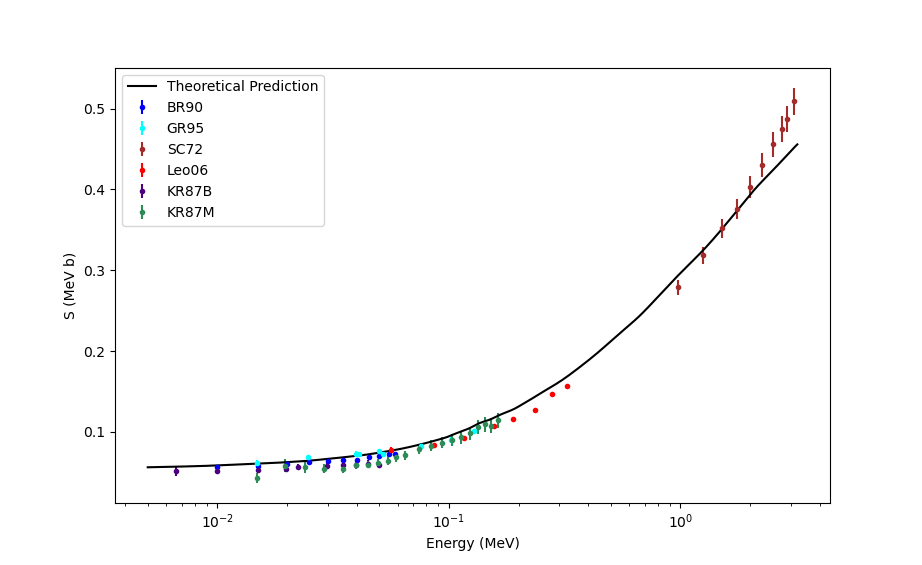
\includegraphics[width=0.6\linewidth]{Figures/ddhe3n_S_theory.png}
	\caption{The theoretical calculation for the $d$($d$,$n$)$^3$He S-factor from \cite{Arai2011} without any scaling. }
\end{figure}

PRIMAT adopt a Bayesian approach to scale the S-factor result from \cite{Arai2011} by some value of order unity to fit the experimental data, since the theory curve lies above nearly all of the experimental data points (see Figure 12). To determine this value, each of the five datasets they use (the collection of datasets in Figure 1 excluding RG85 and SC72) are each scaled by an overall constant to account for the normalization error of each experiment, in addition to the overall scaling. This gives six total parameters to determine in the fit. They use a Metropolis-Hastings MCMC to optimize and sample these parameters. Each dataset scaling parameter has a log-normal prior centered at one with the reported systematic error as the variance. The overall scaling has a non-informative prior, constrained to be positive. The likelihood is the sum of log-normal likelihoods for each datapoint. After burn-in, each S-factor sample is integrated using (2) to get the corresponding rate at 60 temperatures in the range relevant for BBN. The mean rate and variance at each temperature reported are directly obtained from this posterior. The details are slightly different for $d$($p$,$\gamma$)$^3$He, but the overall method is the same (see \cite{Moscoso2021} for more details). 

Both PArthENoPE and PRIMAT compute their mean and 1$\sigma$ rates entirely separately from the BBN calculation. Abundances are calculated by passing the mean rates into each respective BBN code, while the variances are estimated by using their calculated 1$\sigma$ rates. This does not allow for variations in the reaction rate shape allowed by the experimental data. Additionally, both approaches assume a particular functional form for the S-factor and do not vary rates together. 

\bibliography{references}

\end{document}